\section{Evaluation}

\subsection{Experimental Setup}

The implementation mainly consists of two components; the test suite and the sketching algorithms. The entire code-base has been written in Python 3.8. The architecture of the benchmarking test suit is shown in Fig.~\ref{fig:test_suite}. It was designed in a modular way such that it permits easy addition of more test cases and graph sketches when necessary. 

\begin{figure}[htbp]
    \centerline{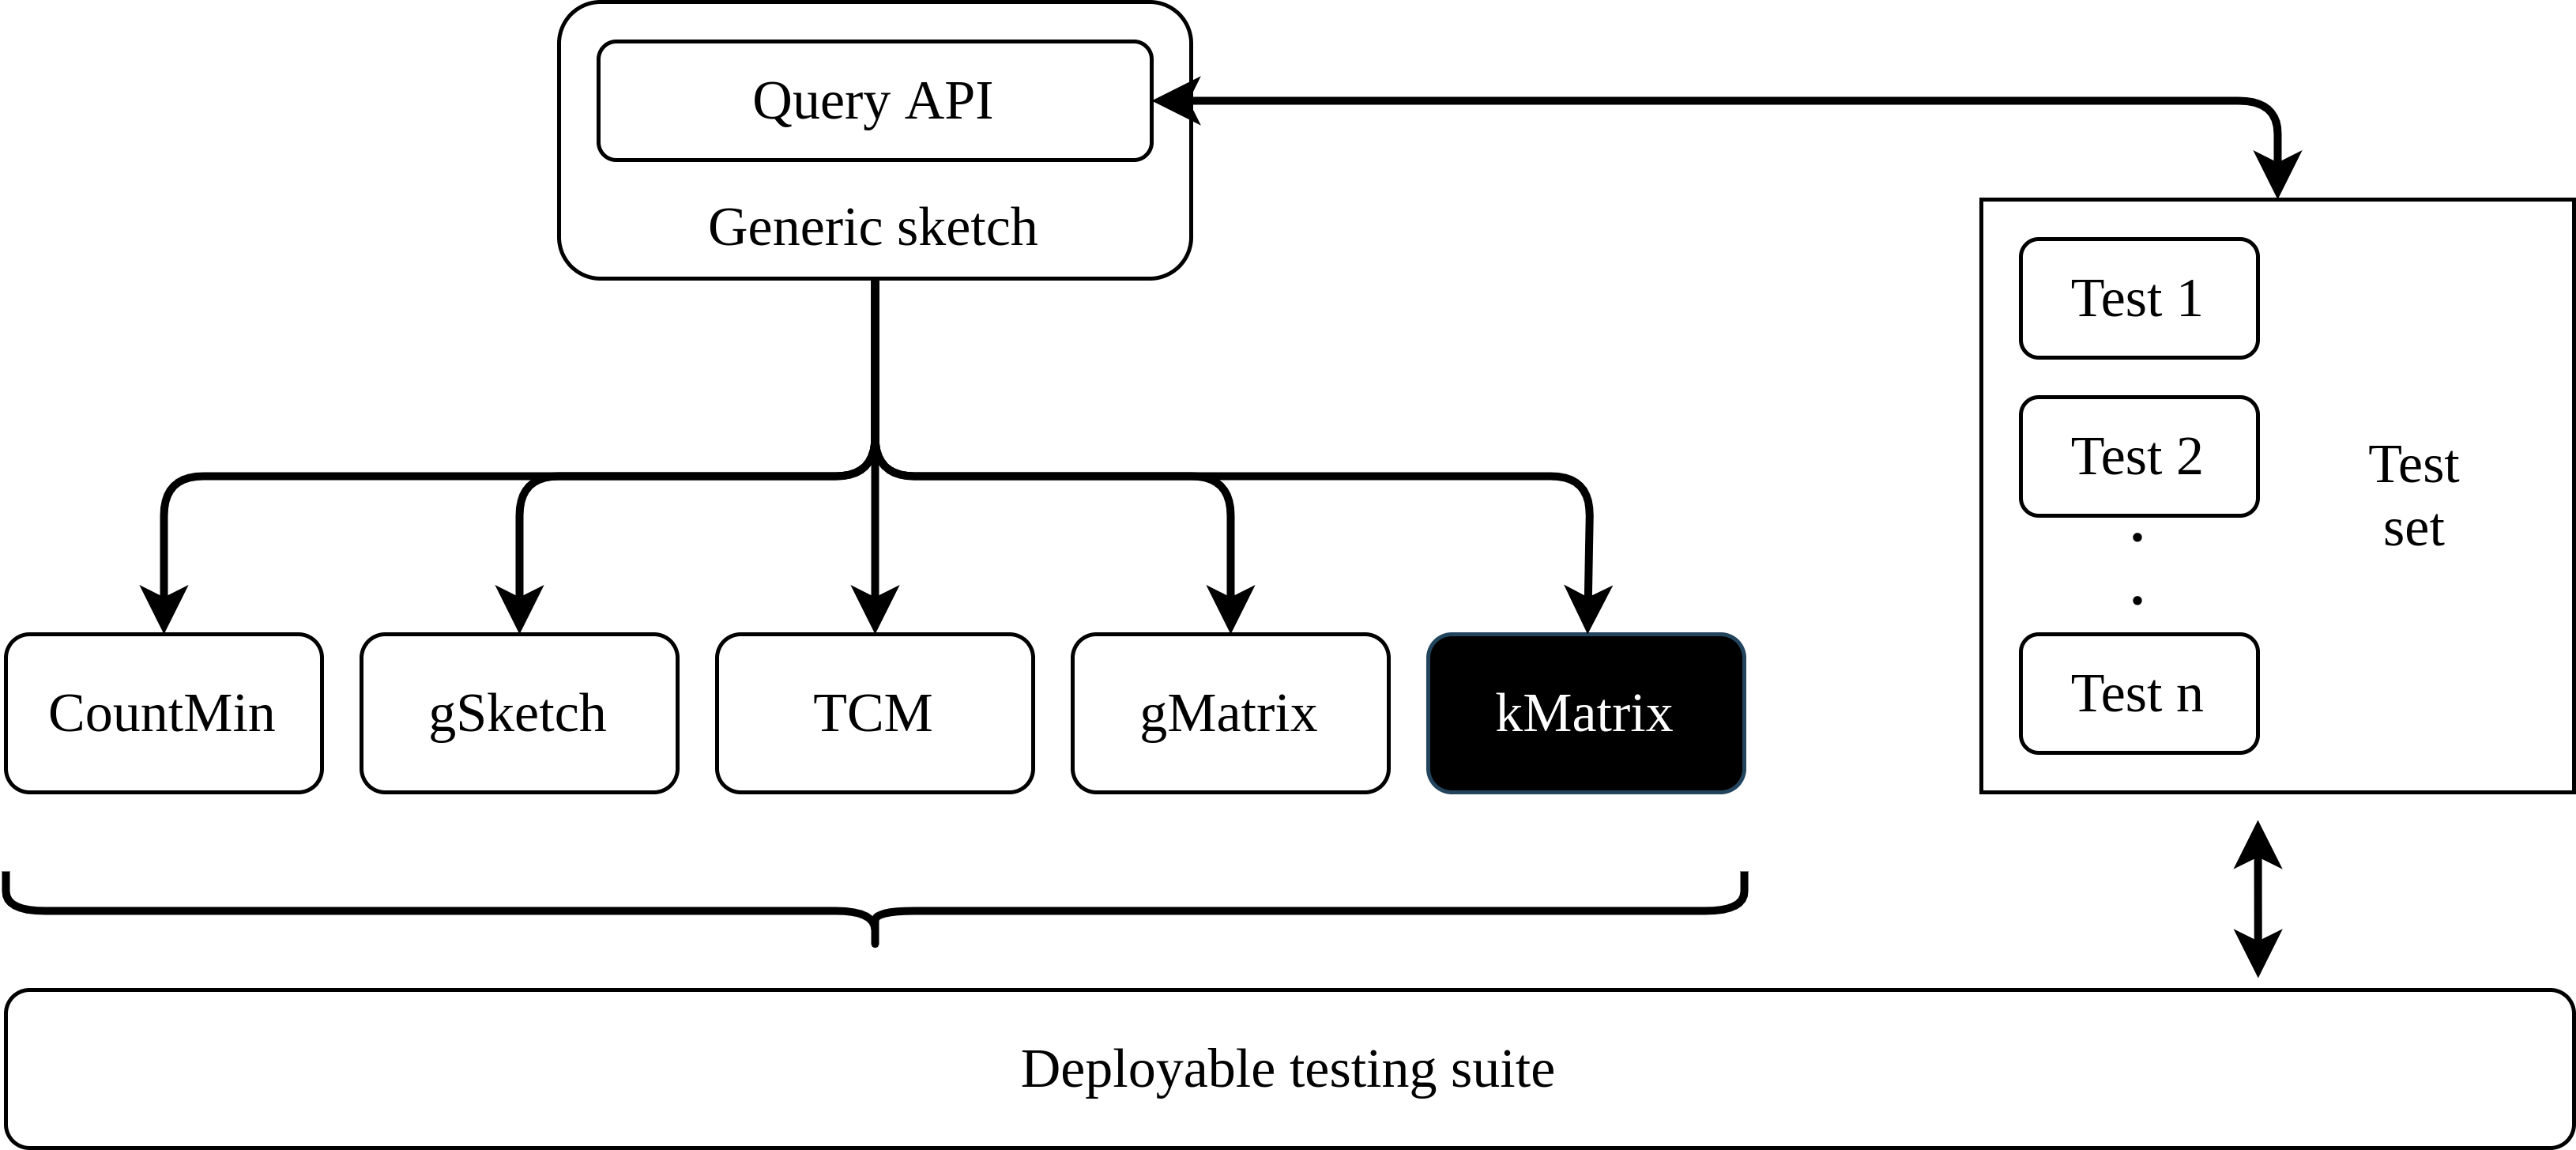
\includegraphics[width=0.5\textwidth]{img/test_suite.png}}
    \caption{High level architecture of the test suite}
    \label{fig:test_suite}
\end{figure}

All the tests were run on a 12-core Ryzen 3900 machine with a base clock of 3.1GHz and 32 GB RAM. However, only one core was utilized in running the tests.

A sample of 30,000 edges has been extracted from relevant datasets for initializing kMatrix at the beginning of each experiment. This sample stream has been obtained using reservoir sampling. 

\subsection{Datasets}

3 datasets were chosen to carry out the benchmarking process in this research. These were chosen to represent different application domains. 

\paragraph{unicorn-wget\cite{DVN/5H4TDI_2018}}
unicorn-wget is a dataset created from capturing the packet information of the network activity of a simulated network. This dataset was created at Harvard University. The dataset consists of 5 parts. From them, Hour-Long Wget Benign Dataset (Base Graph) which consist of 17,778 nodes and 2,779,726 edges was chosen for the experiment. We filtered 10\% of the edges using reservoir sampling for our experiments. 

\paragraph{email-EuAll\cite{leskovec_graph_2007}}
This data was extracted using email data from a large European research institution. The dataset consists of emails sent out in a period of 18 months. Each data item contains sender, receiver and the time of the origination of each email. The dataset consisted of 265,214 nodes and 420,045 edges\cite{noauthor_snap_nodate_email}. 

\paragraph{cit-HepPh\cite{leskovec_graphs_2005, gehrke_overview_2003}}
cit-HepPh citation graph is from the e-print arXiv regarding high energy physics phenomenology. It has 34,546 papers (nodes) and 421,578 citations (edges). We used the full dataset in our experiments. 

\subsection{Evaluation Metrics}
\label{section:design_evaluation_metrics}

\subsubsection{Average Relative Error (ARE)}
\label{section:metrics_are}

The average relative error is defined as,

\begin{equation}
    er(Q) =  \frac{\tilde{f}'(Q) - f(Q)}{f(Q)} = \frac{\tilde{f}'(Q)}{f(Q)} -1
\end{equation}

Given a set of m queries, $\{ Q_1 , ....., Q_m \}$, the average relative error is defined by taking the average of the relative error of all queries $Q_i$ for \(i \in [1,m]\).

\begin{equation}
    e(Q) =  \frac{\sum_{i=1}^{k} er(Q_i)}{m}
\end{equation}

\subsubsection{Number of Effective Queries (NEQ)}
\label{section:metrics_neq}

A query is said to be effective if the error, $\tilde{f}'(Q) - f(Q), < G_0$,  where $G_0$ is a predefined value. The number of effective queries is defined as,

\begin{equation}
    g(Q) =  \left | \{\,q\, |   \left |\tilde{f}'(q) - f(q)\right | \leq G_0, \,q \, \epsilon  \,Q\} \, \right|
\end{equation}

This can also be expressed as a percentage of effective queries (PEQ).

\begin{equation}
    g(Q) =  \frac{\left | \{\,q\, |   \left |\tilde{f}'(q) - f(q)\right | \leq G_0, \,q \, \epsilon  \,Q\} \, \right|}{|Q|}*100
\end{equation}

\subsection{Results}

This section will describe all the experiments conducted to measure the effectiveness of kMatrix against existing streaming graph sketching techniques. 

We have considered CountMin, gSketch, TCM, gMatrix and kMatrix sketches in our experiments. These sketches can be categorized into two groups depending on the type of queries they are able to answer.

\begin{enumerate}
    \item \emph{Type I} - The sketches which support only the edge frequency queries, i.e. CountMin and gSketch.
    \item \emph{Type II} - The sketches which support many graph queries in general, i.e. TCM, gMatrix and kMatrix
\end{enumerate}

Since \emph{Type I} sketches cannot answer anything other than edge frequency queries, we have only included \emph{Type II} sketches in our comparisons against kMatrix.

\subsection{Build-time}

Here we investigated the time to add the entire dataset to the sketch. The sketches were allocated a constant memory size of 1 MB, and the number of hash functions was set to \(d = 7\). The edges were streamed at the maximum throughput of each sketch. Therefore this experiment gives an idea about the average insertion rate of edges for each sketch. A minor drawback of kMatrix is that it takes some time for its initialization stage. However, this initialization time becomes negligible compared to the advantage that kMatrix receives over time due to its faster streaming rate. In both Fig.~\ref{fig:btt-a} and Fig.~\ref{fig:btt-c}, it has managed to outperform other sketching techniques by a significant margin. In Fig.~\ref{fig:btt-b}, kMatrix has shown comparable performance to gMatrix.

\begin{figure}[htbp] 
    \centering
    \subfloat[unicorn-wget\label{fig:btt-a}]{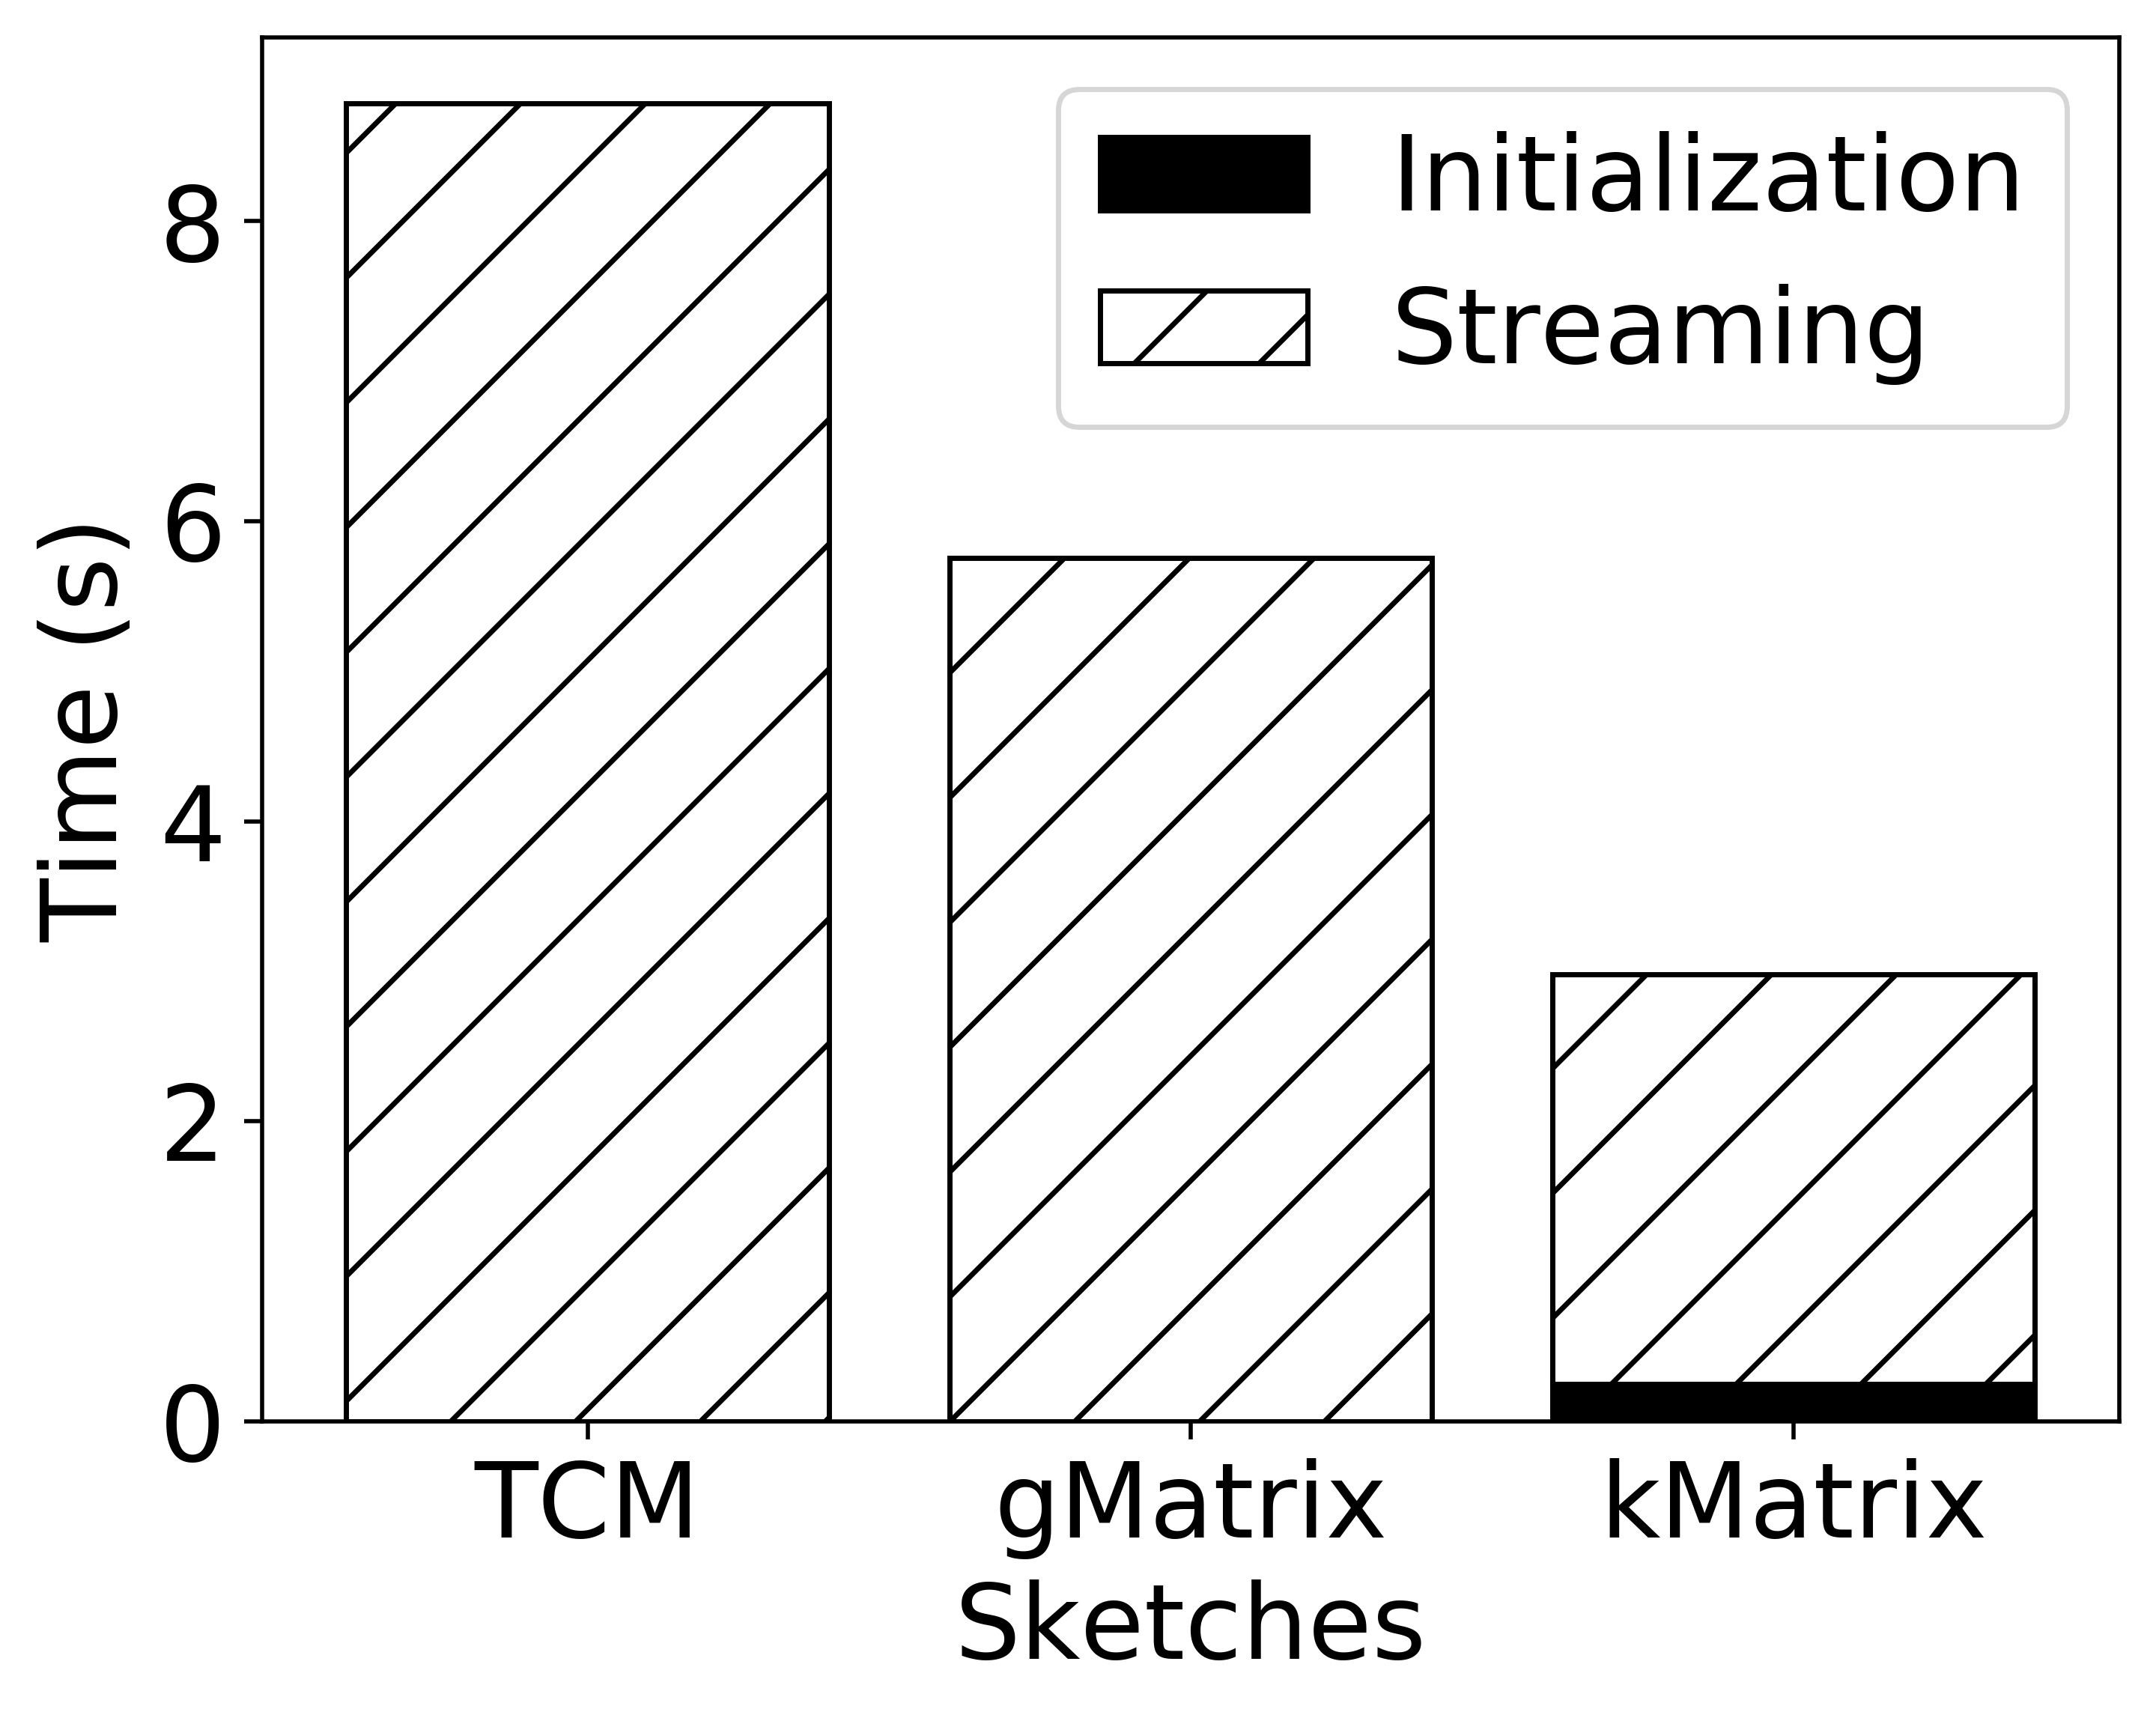
\includegraphics[width=0.45\linewidth]{img/buildtime_1024_unicorn-wget.png}}
    \hfill
    \subfloat[email-EuAll\label{fig:btt-b}]{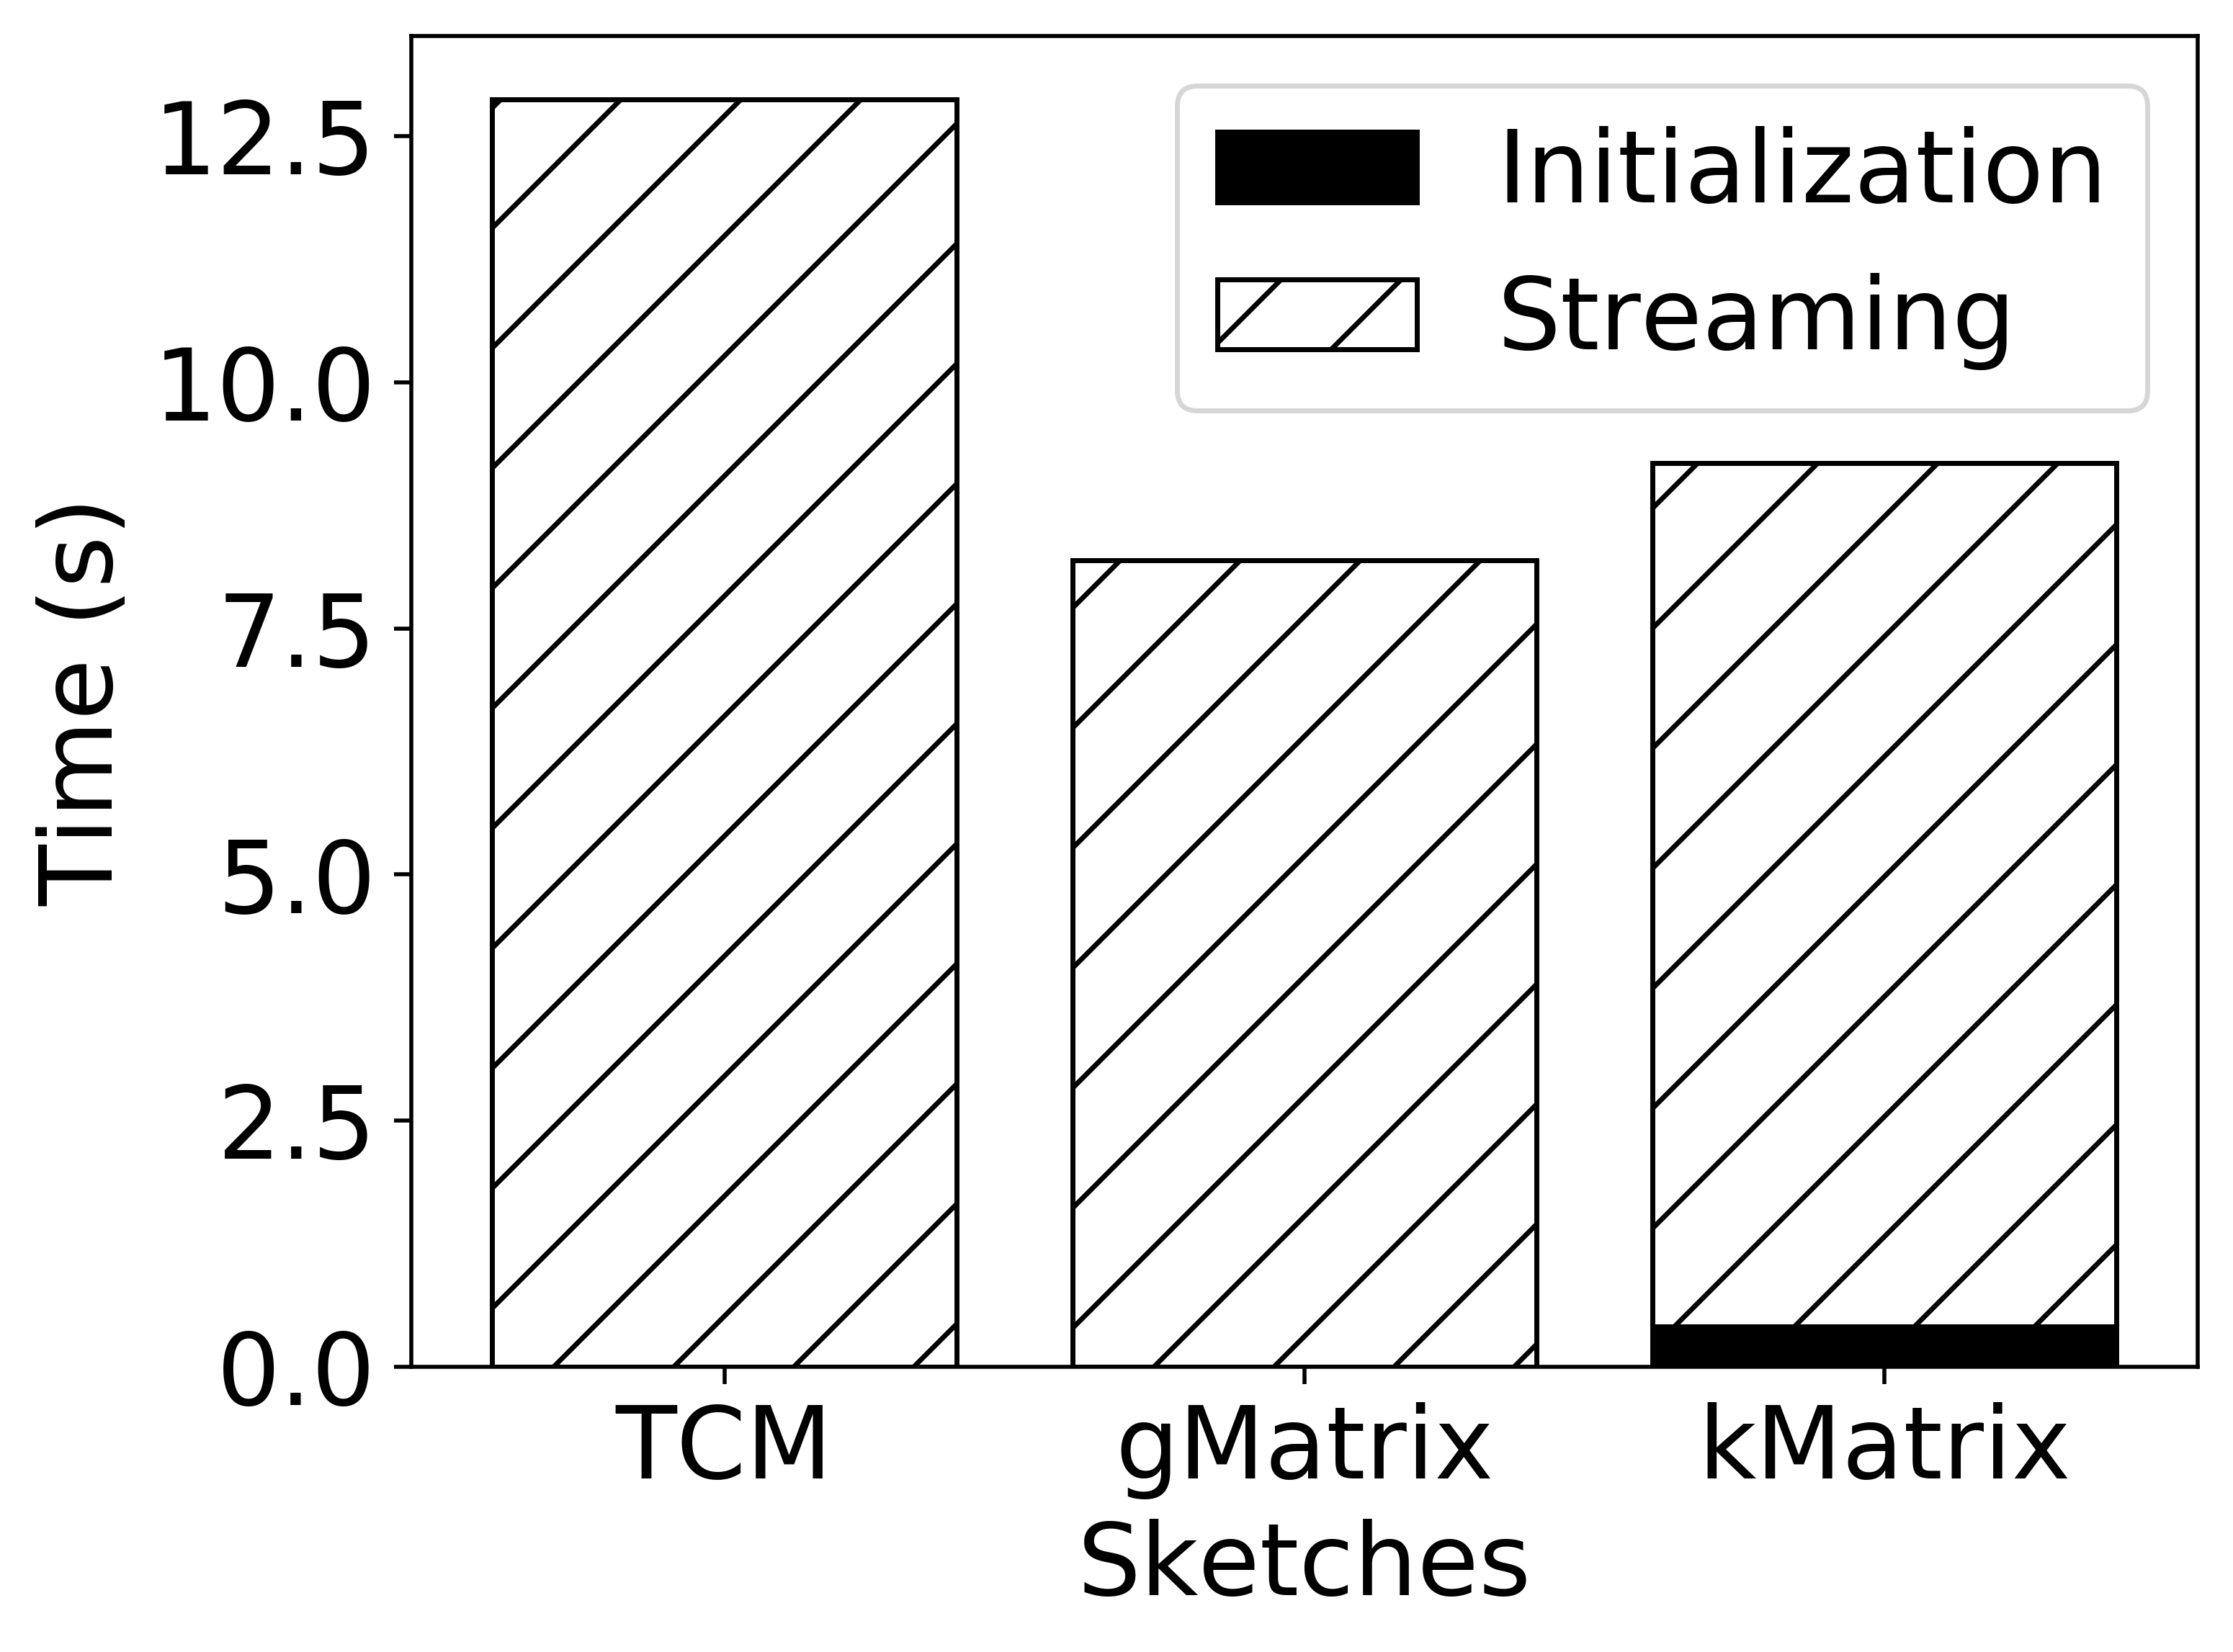
\includegraphics[width=0.45\linewidth]{img/buildtime_1024_email-EuAll.png}}
    \hfill
    \subfloat[cit-HepPh\label{fig:btt-c}]{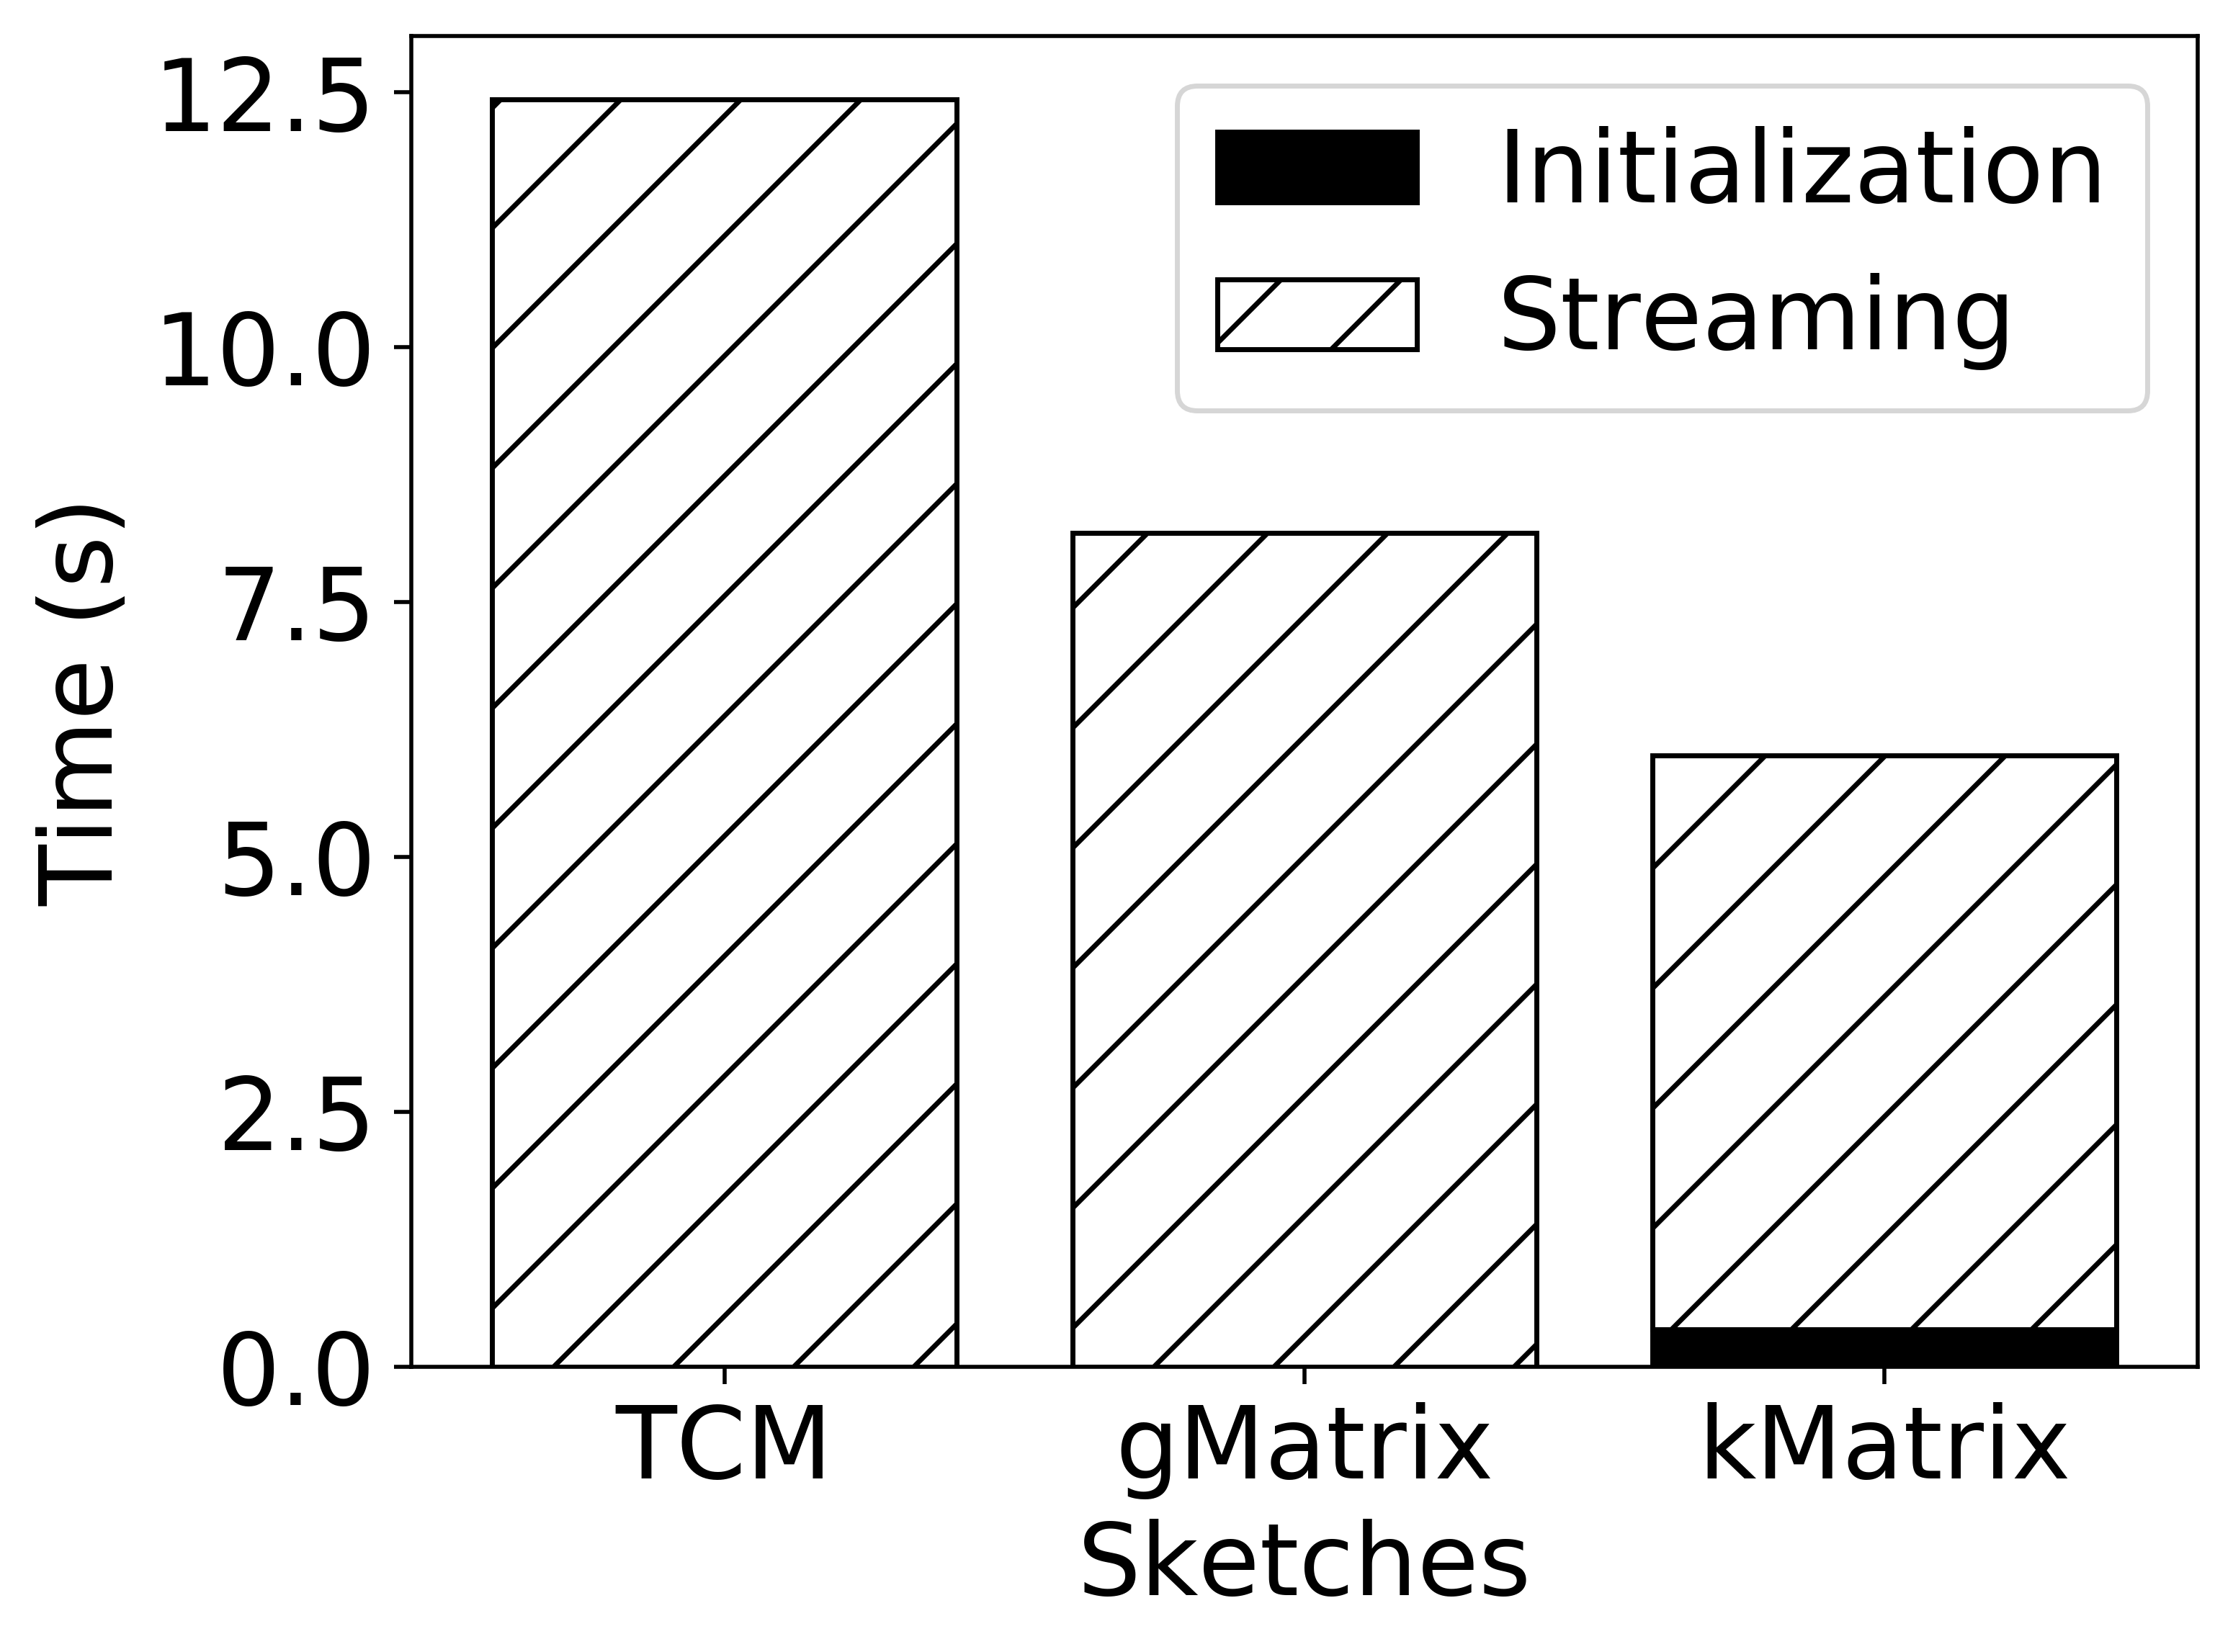
\includegraphics[width=0.45\linewidth]{img/buildtime_1024_cit-HepPh.png}}
    \caption{Build-time}
    \label{fig:buildtime-test}
\end{figure}

\subsection{Edge queries}

This experiment investigates how accurately the kMatrix can answer the edge queries after the summarization process. For this, we let our datastream get summarized into the sketch and then queried the frequency of different edges chosen at random. The experiment was repeated for each sketch for the sizes, 200 KB, 300 KB, 400 KB and 512 KB while keeping the number of hash functions at \(d = 7\). We have used average relative error and the number of effective queries as the evaluation matrices for this experiment.

\subsubsection{Average Relative Error}
\label{section:results_are}

\begin{figure}[htbp] 
    \centering
    \subfloat[unicorn-wget\label{fig:are-a}]{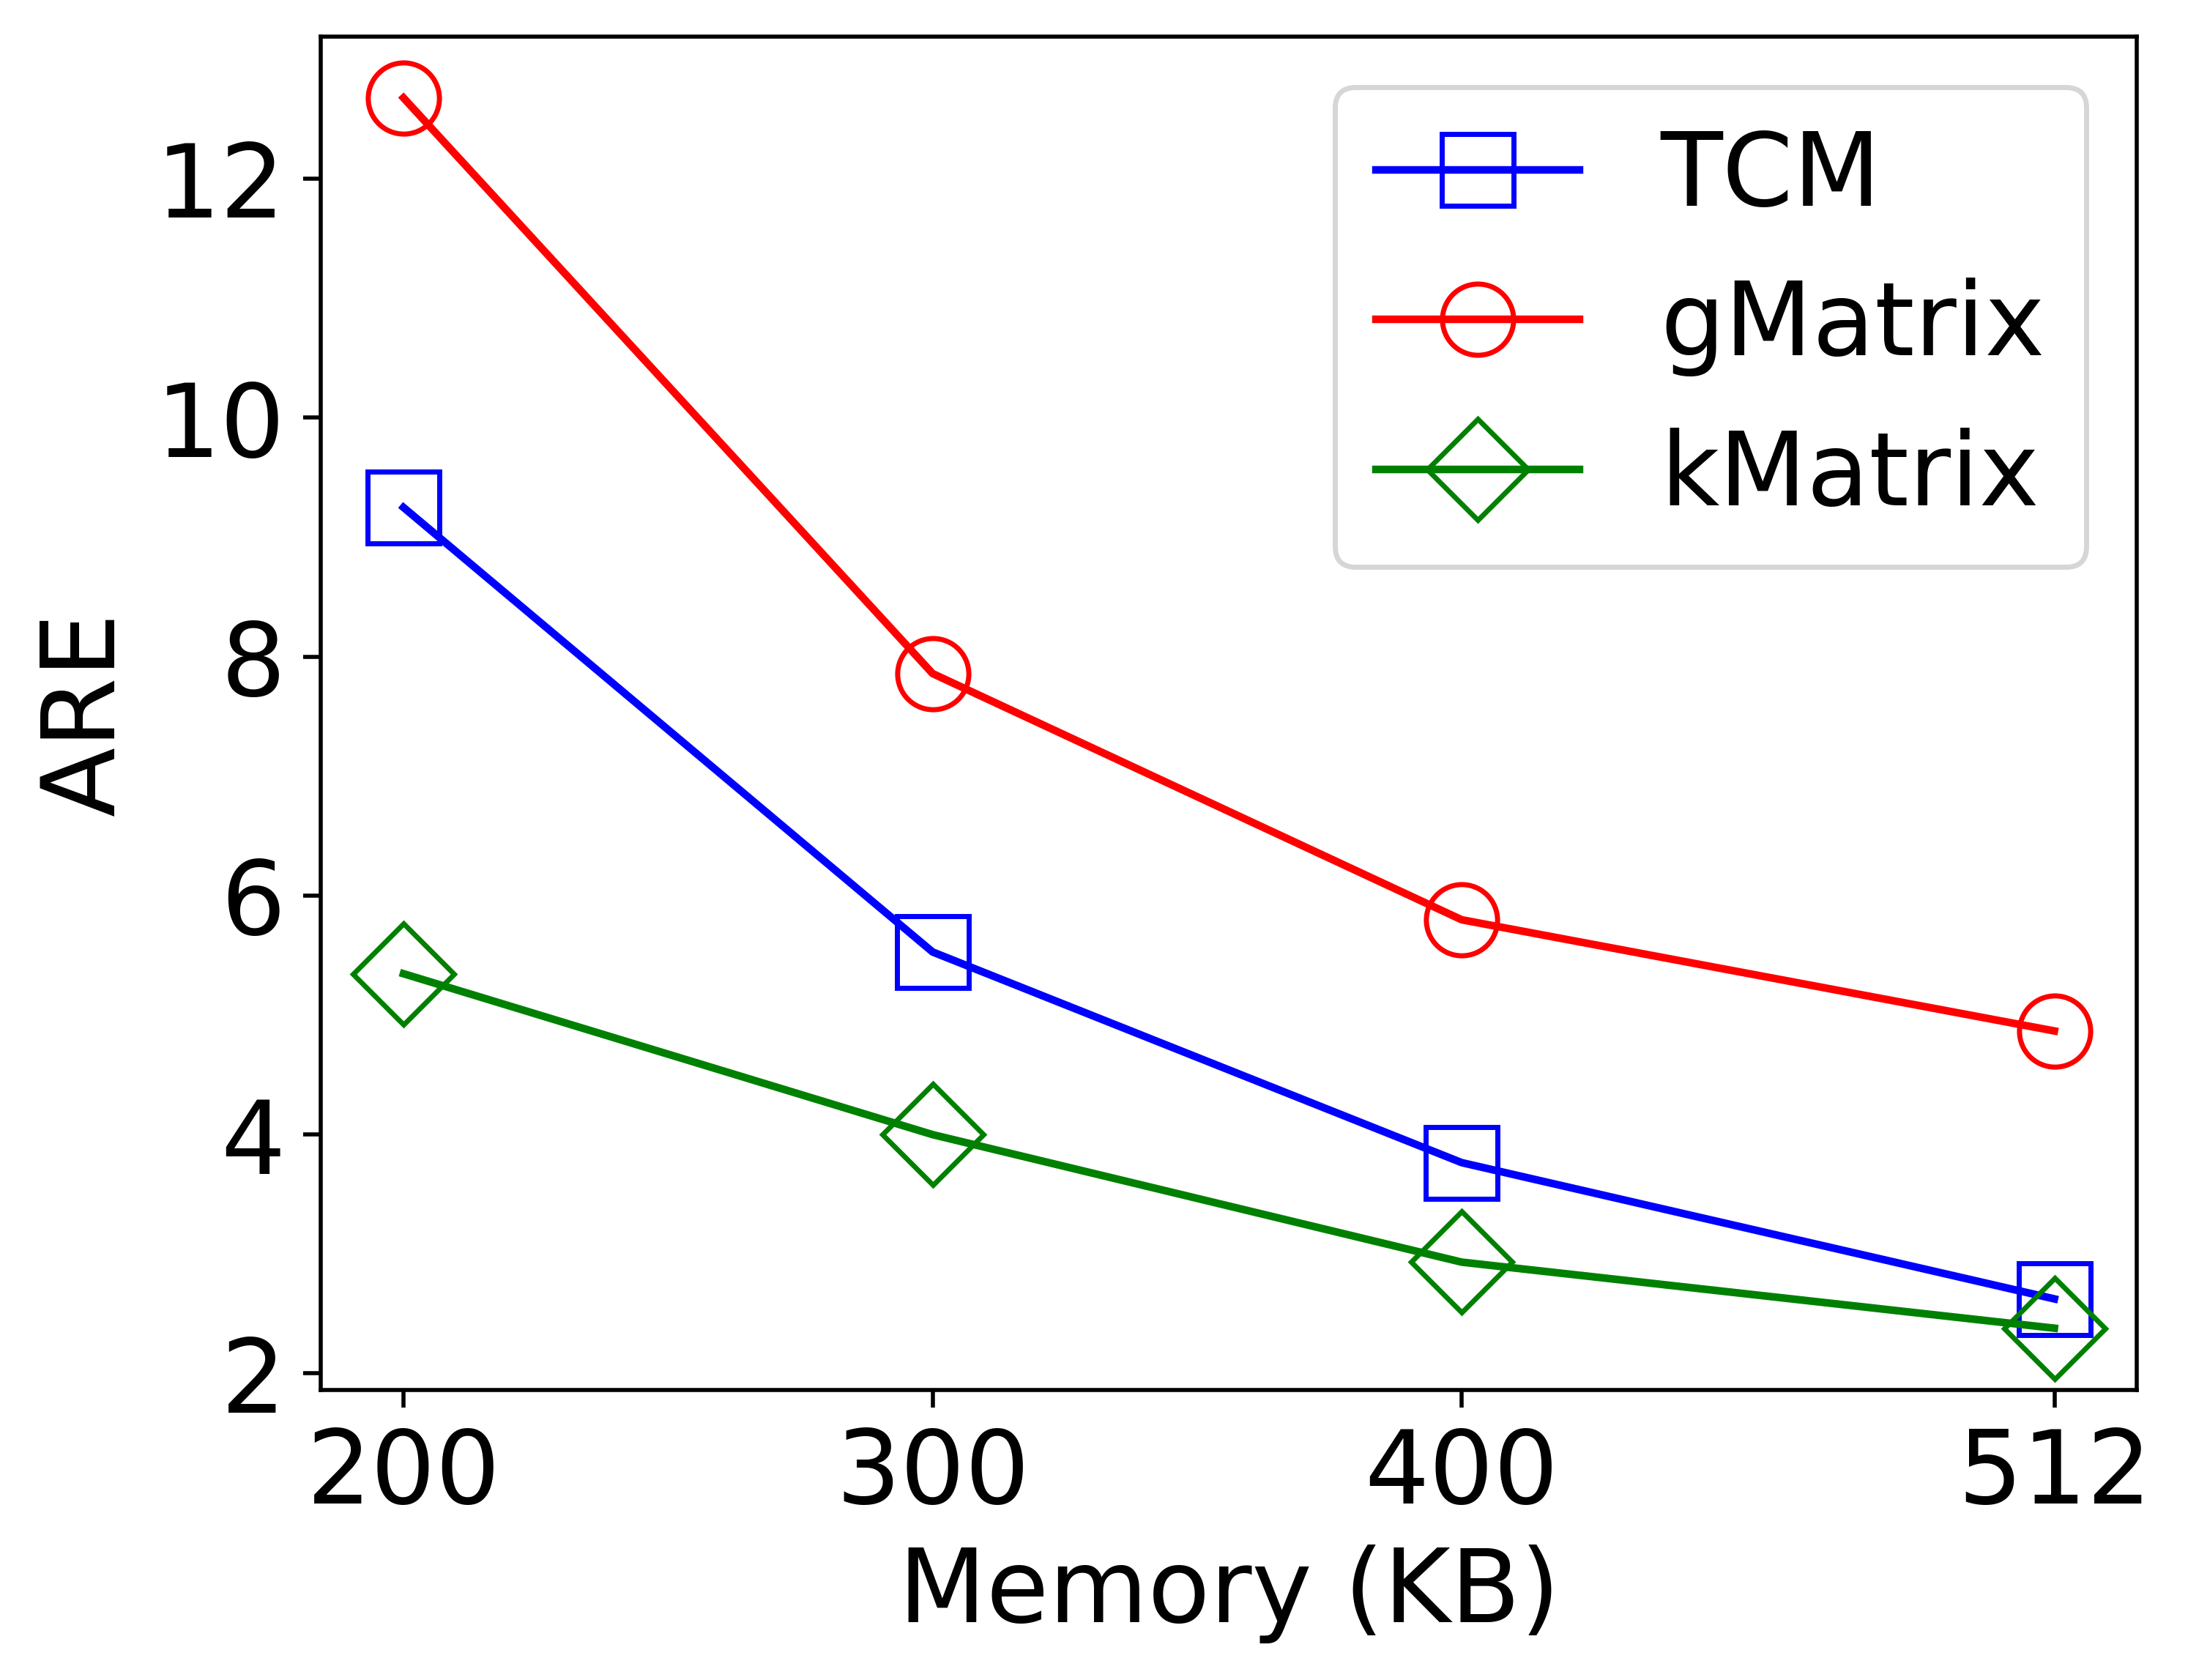
\includegraphics[width=0.45\linewidth]{img/edge_query_are_unicorn-wget.png}}
    \hfill
    \subfloat[email-EuAll\label{fig:are-b}]{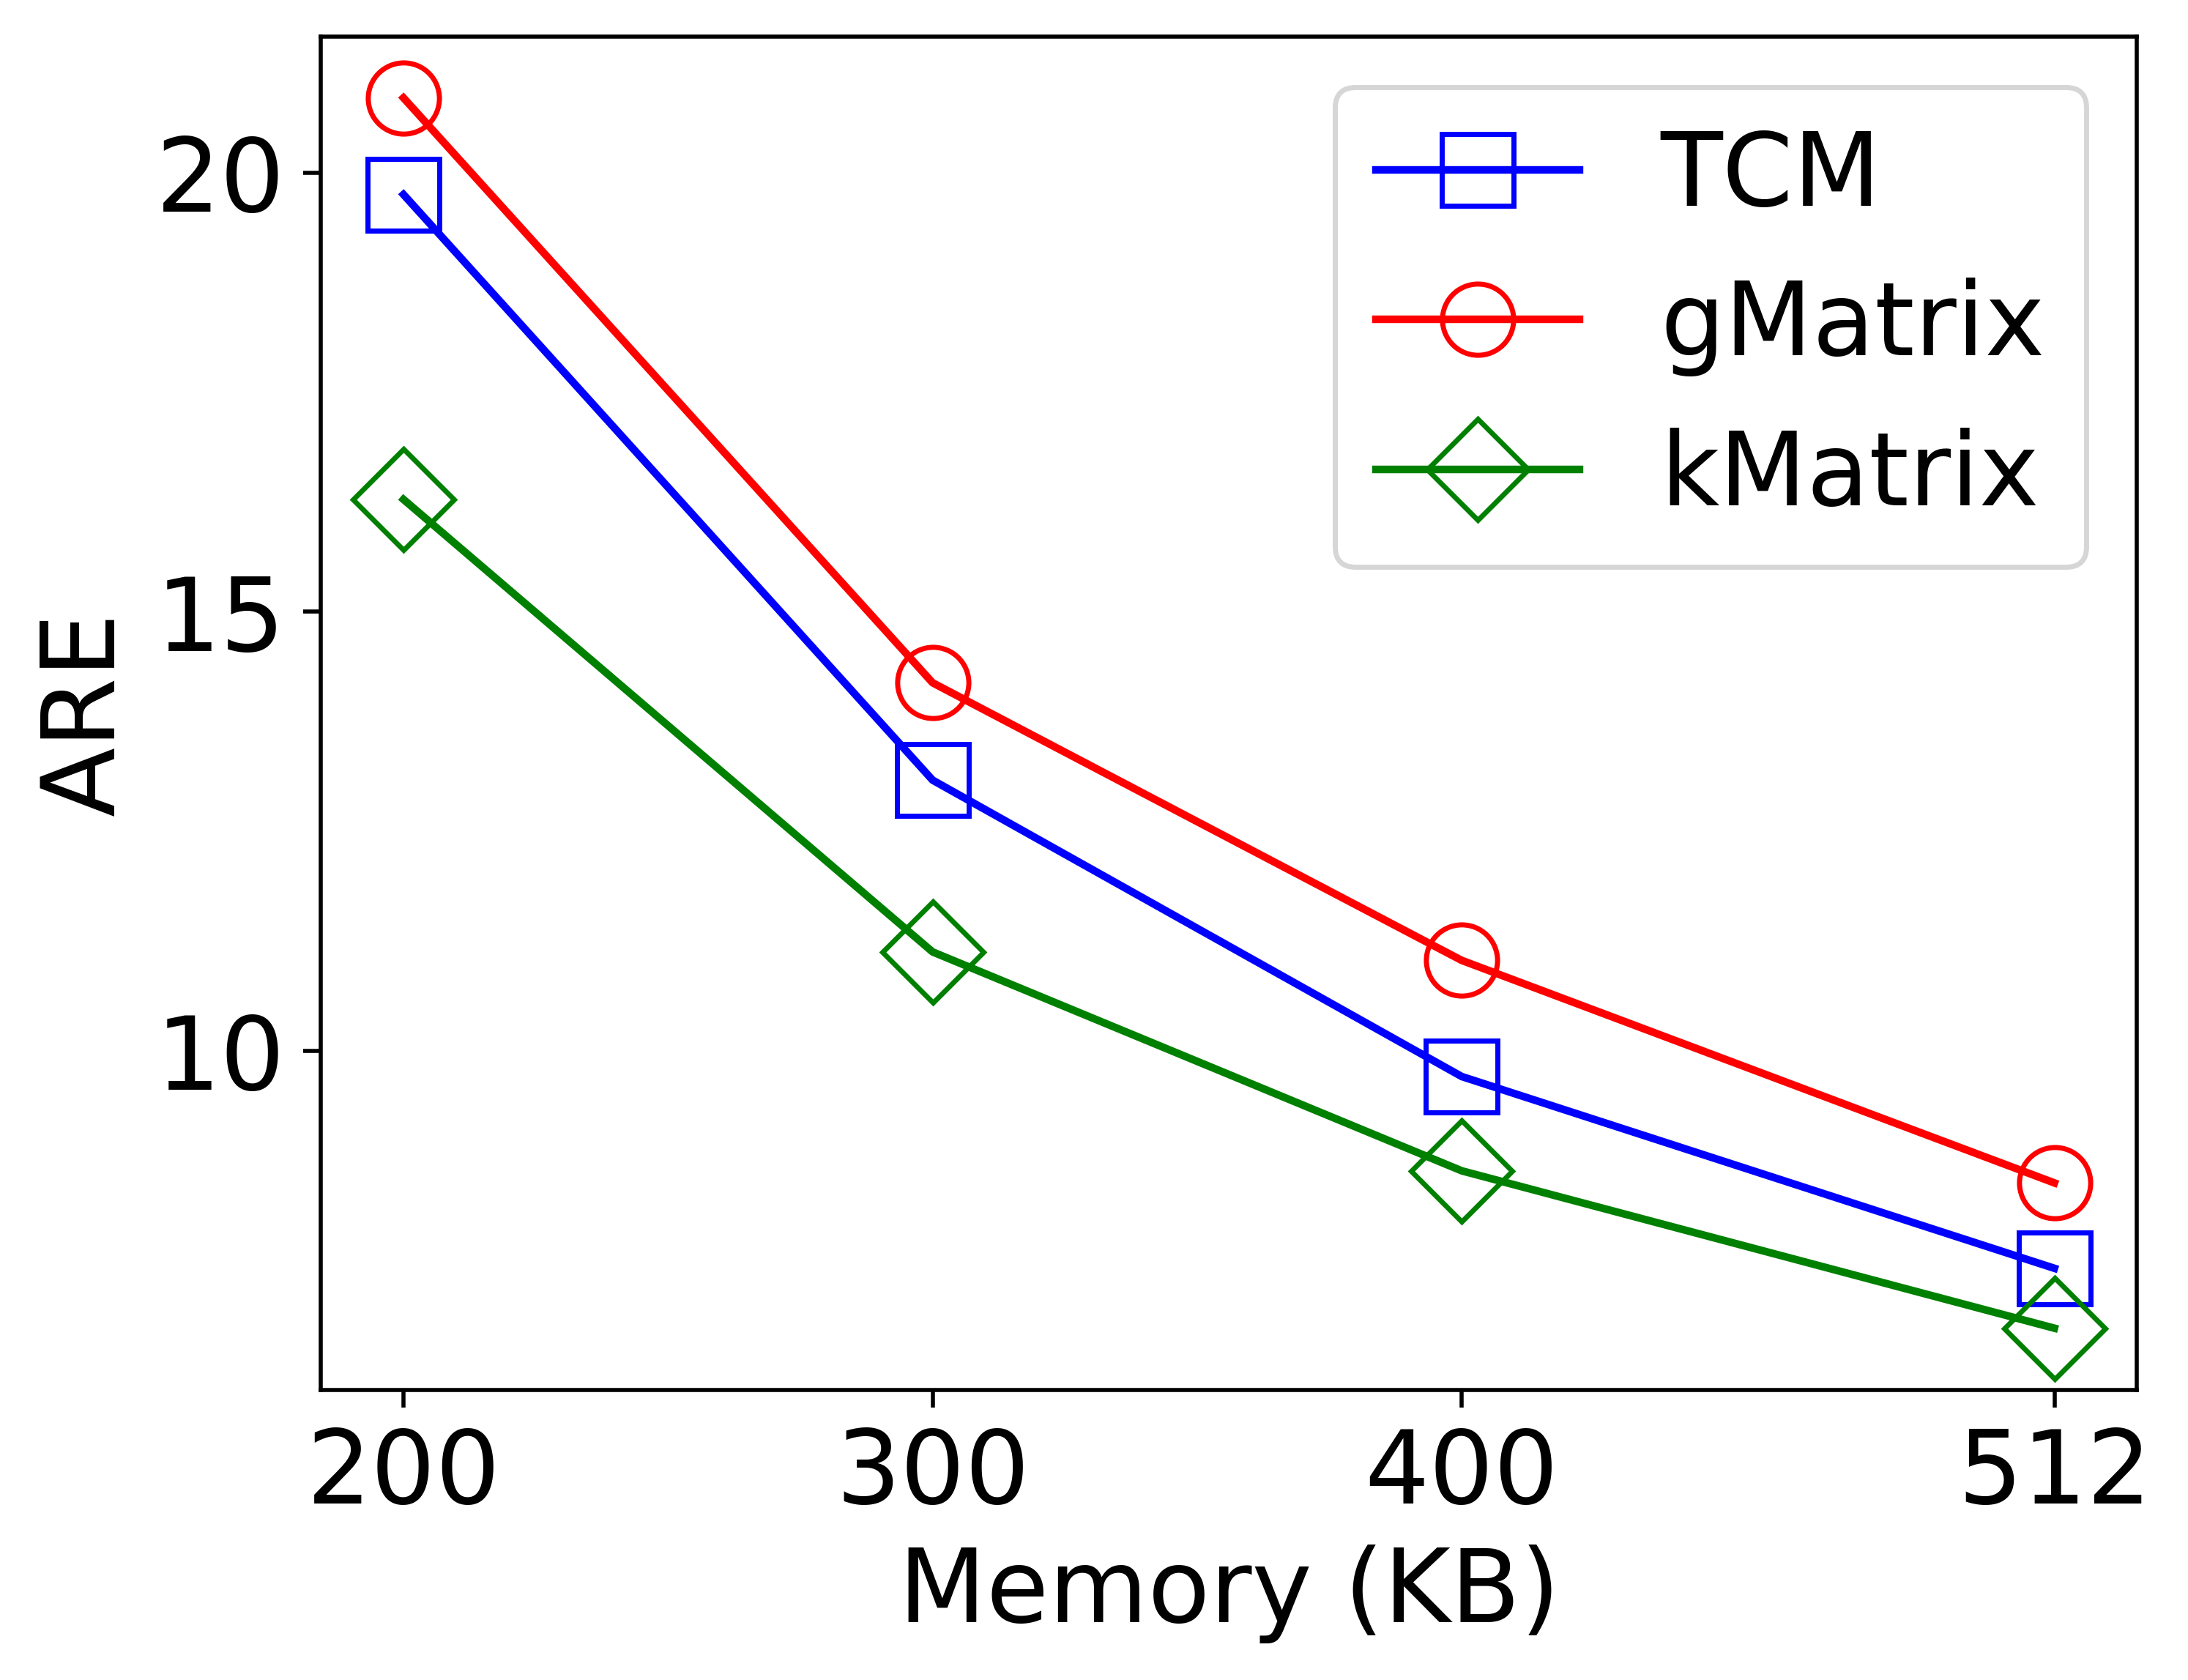
\includegraphics[width=0.45\linewidth]{img/edge_query_are_email-EuAll.png}}
    \hfill
    \subfloat[cit-HepPh\label{fig:are-c}]{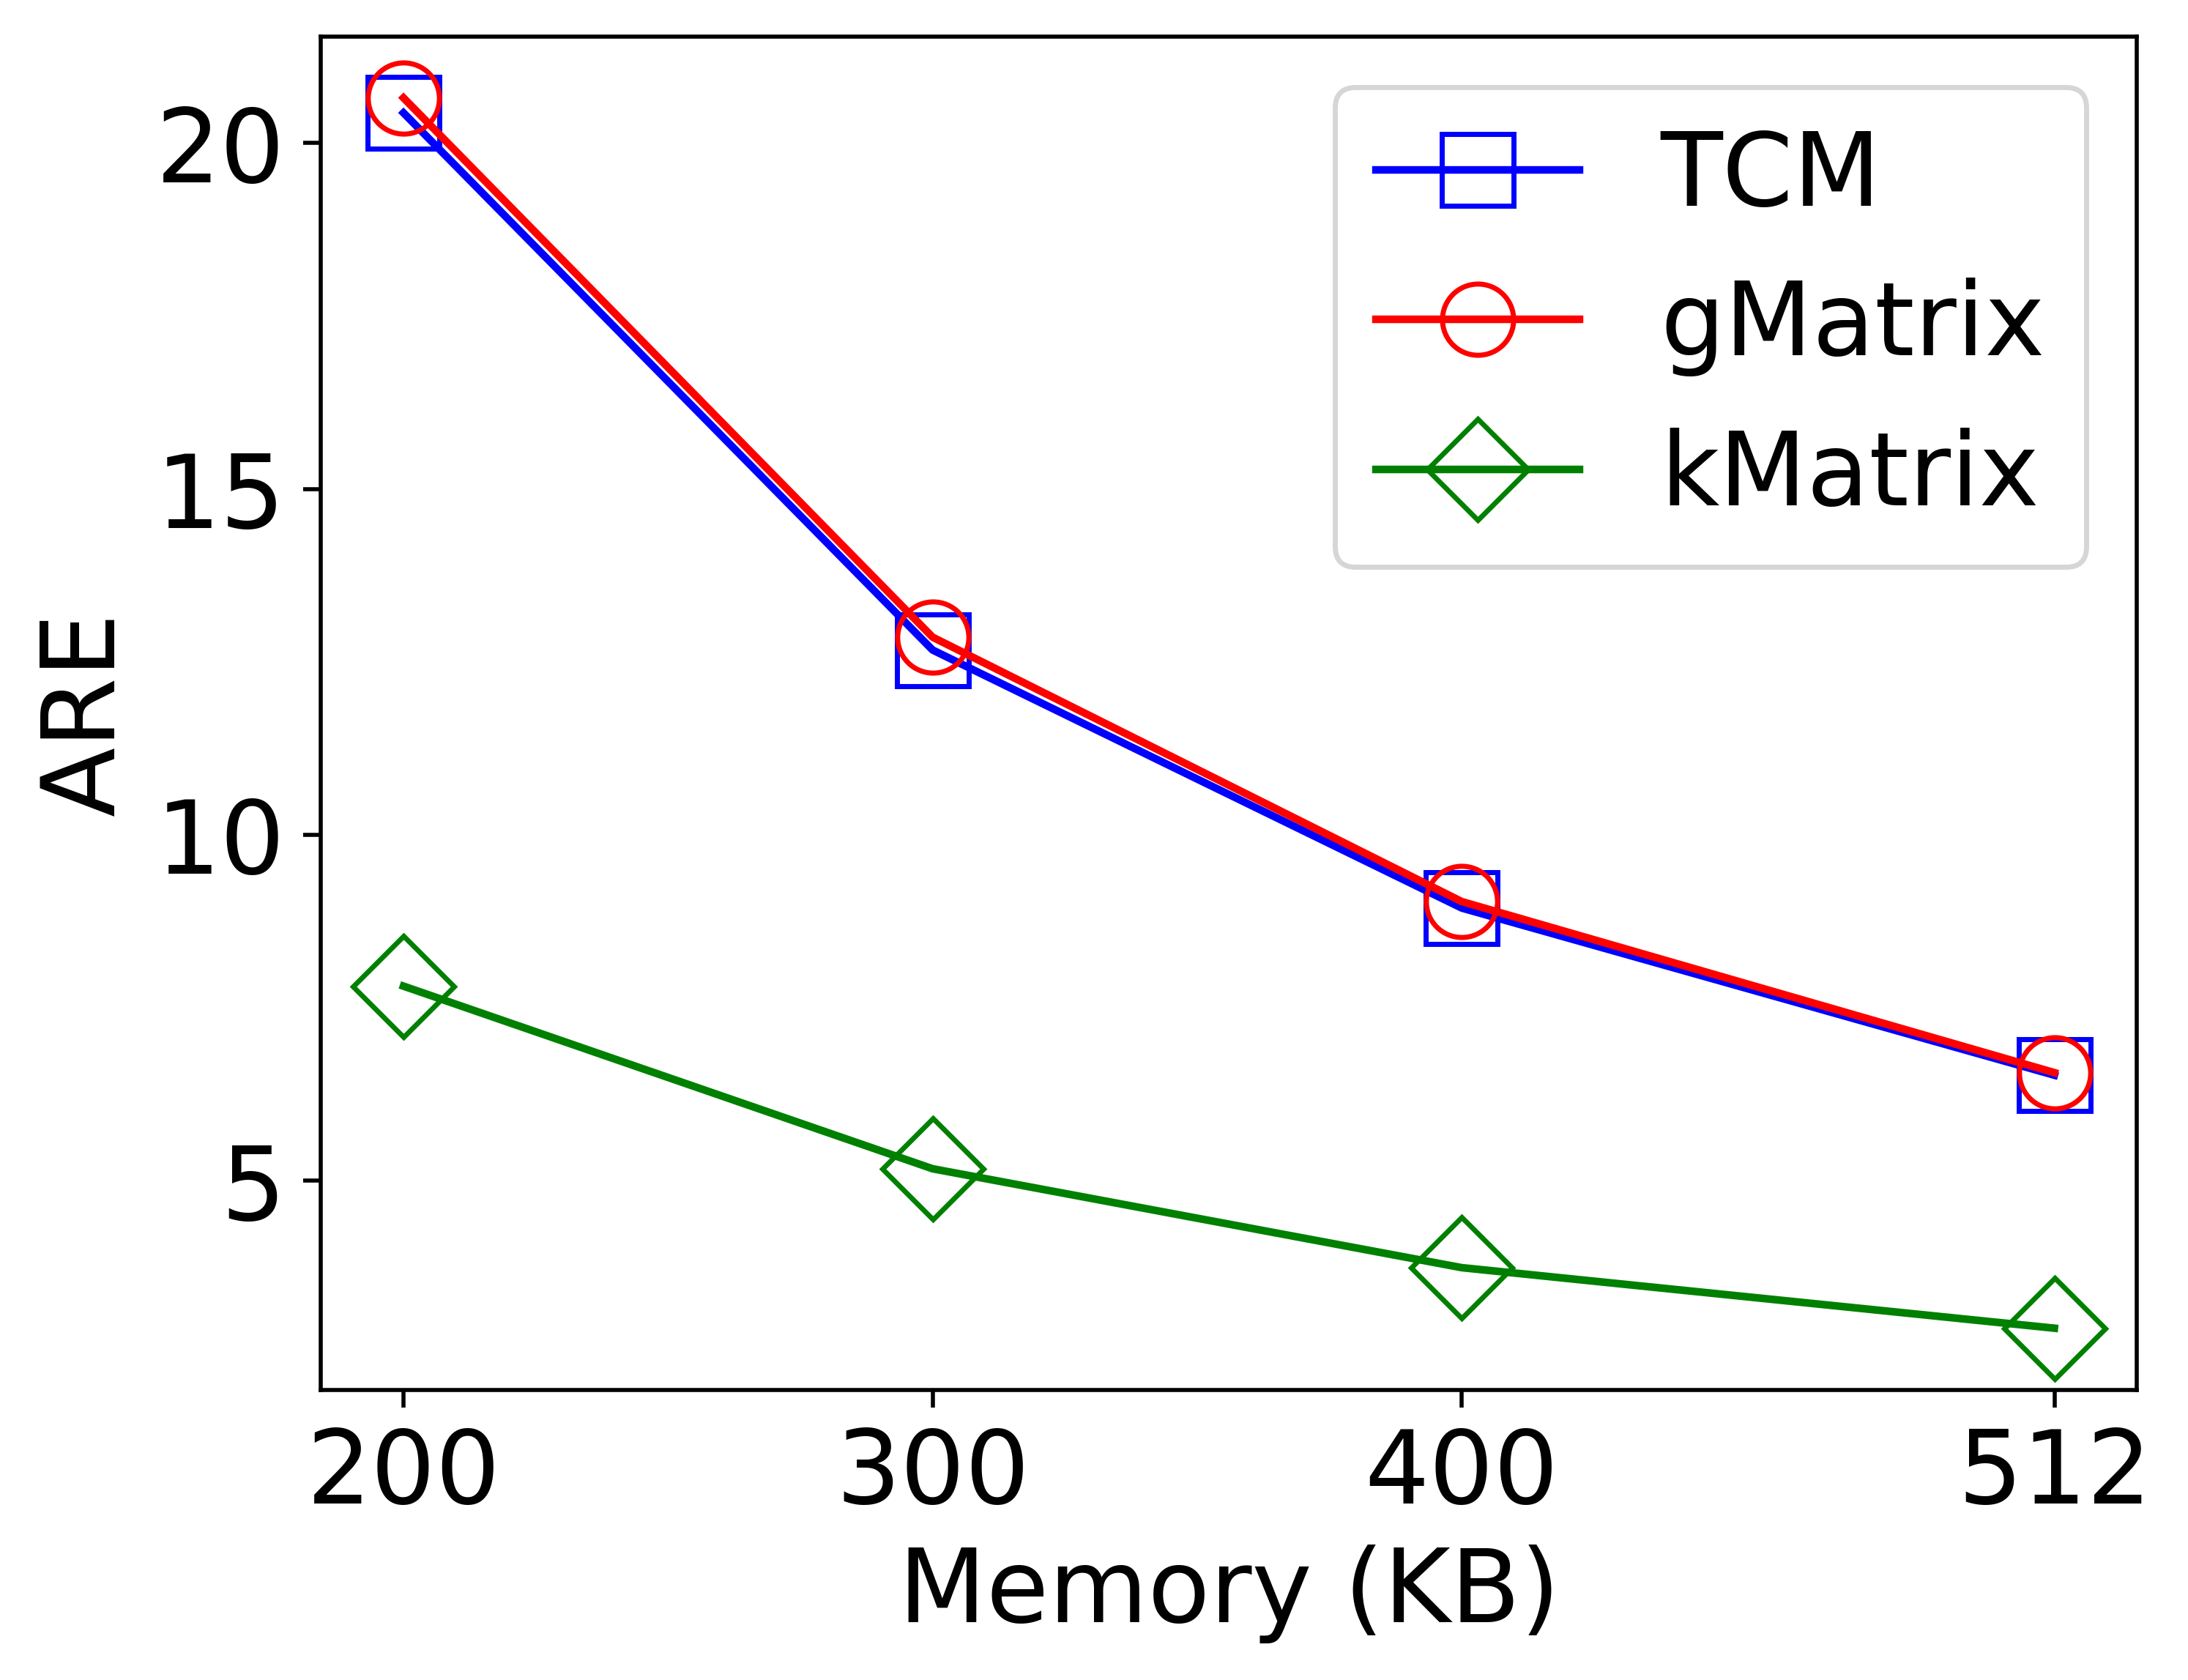
\includegraphics[width=0.45\linewidth]{img/edge_query_are_cit-HepPh.png}}
    \caption{Average relative error}
    \label{fig:edgq-queries-are-test}
\end{figure}

kMatrix showed significantly low ARE than all the other sketches for the three datasets we chose. The reason is that kMatrix can maintain frequency uniformity within each partition, making kMatrix relatively more immune to hash collisions than TCM and gMatrix. It is clear from the experimental evidence shown in Fig.~\ref{fig:edgq-queries-are-test} that kMatrix vastly outperforms the other state of the art sketching techniques. The superiority of our solution is more apparent when the allocated memory is low.

\subsubsection{Number of Effective Queries}

\begin{figure}[htbp] 
    \centering
    \subfloat[unicorn-wget\label{fig:neq-a}]{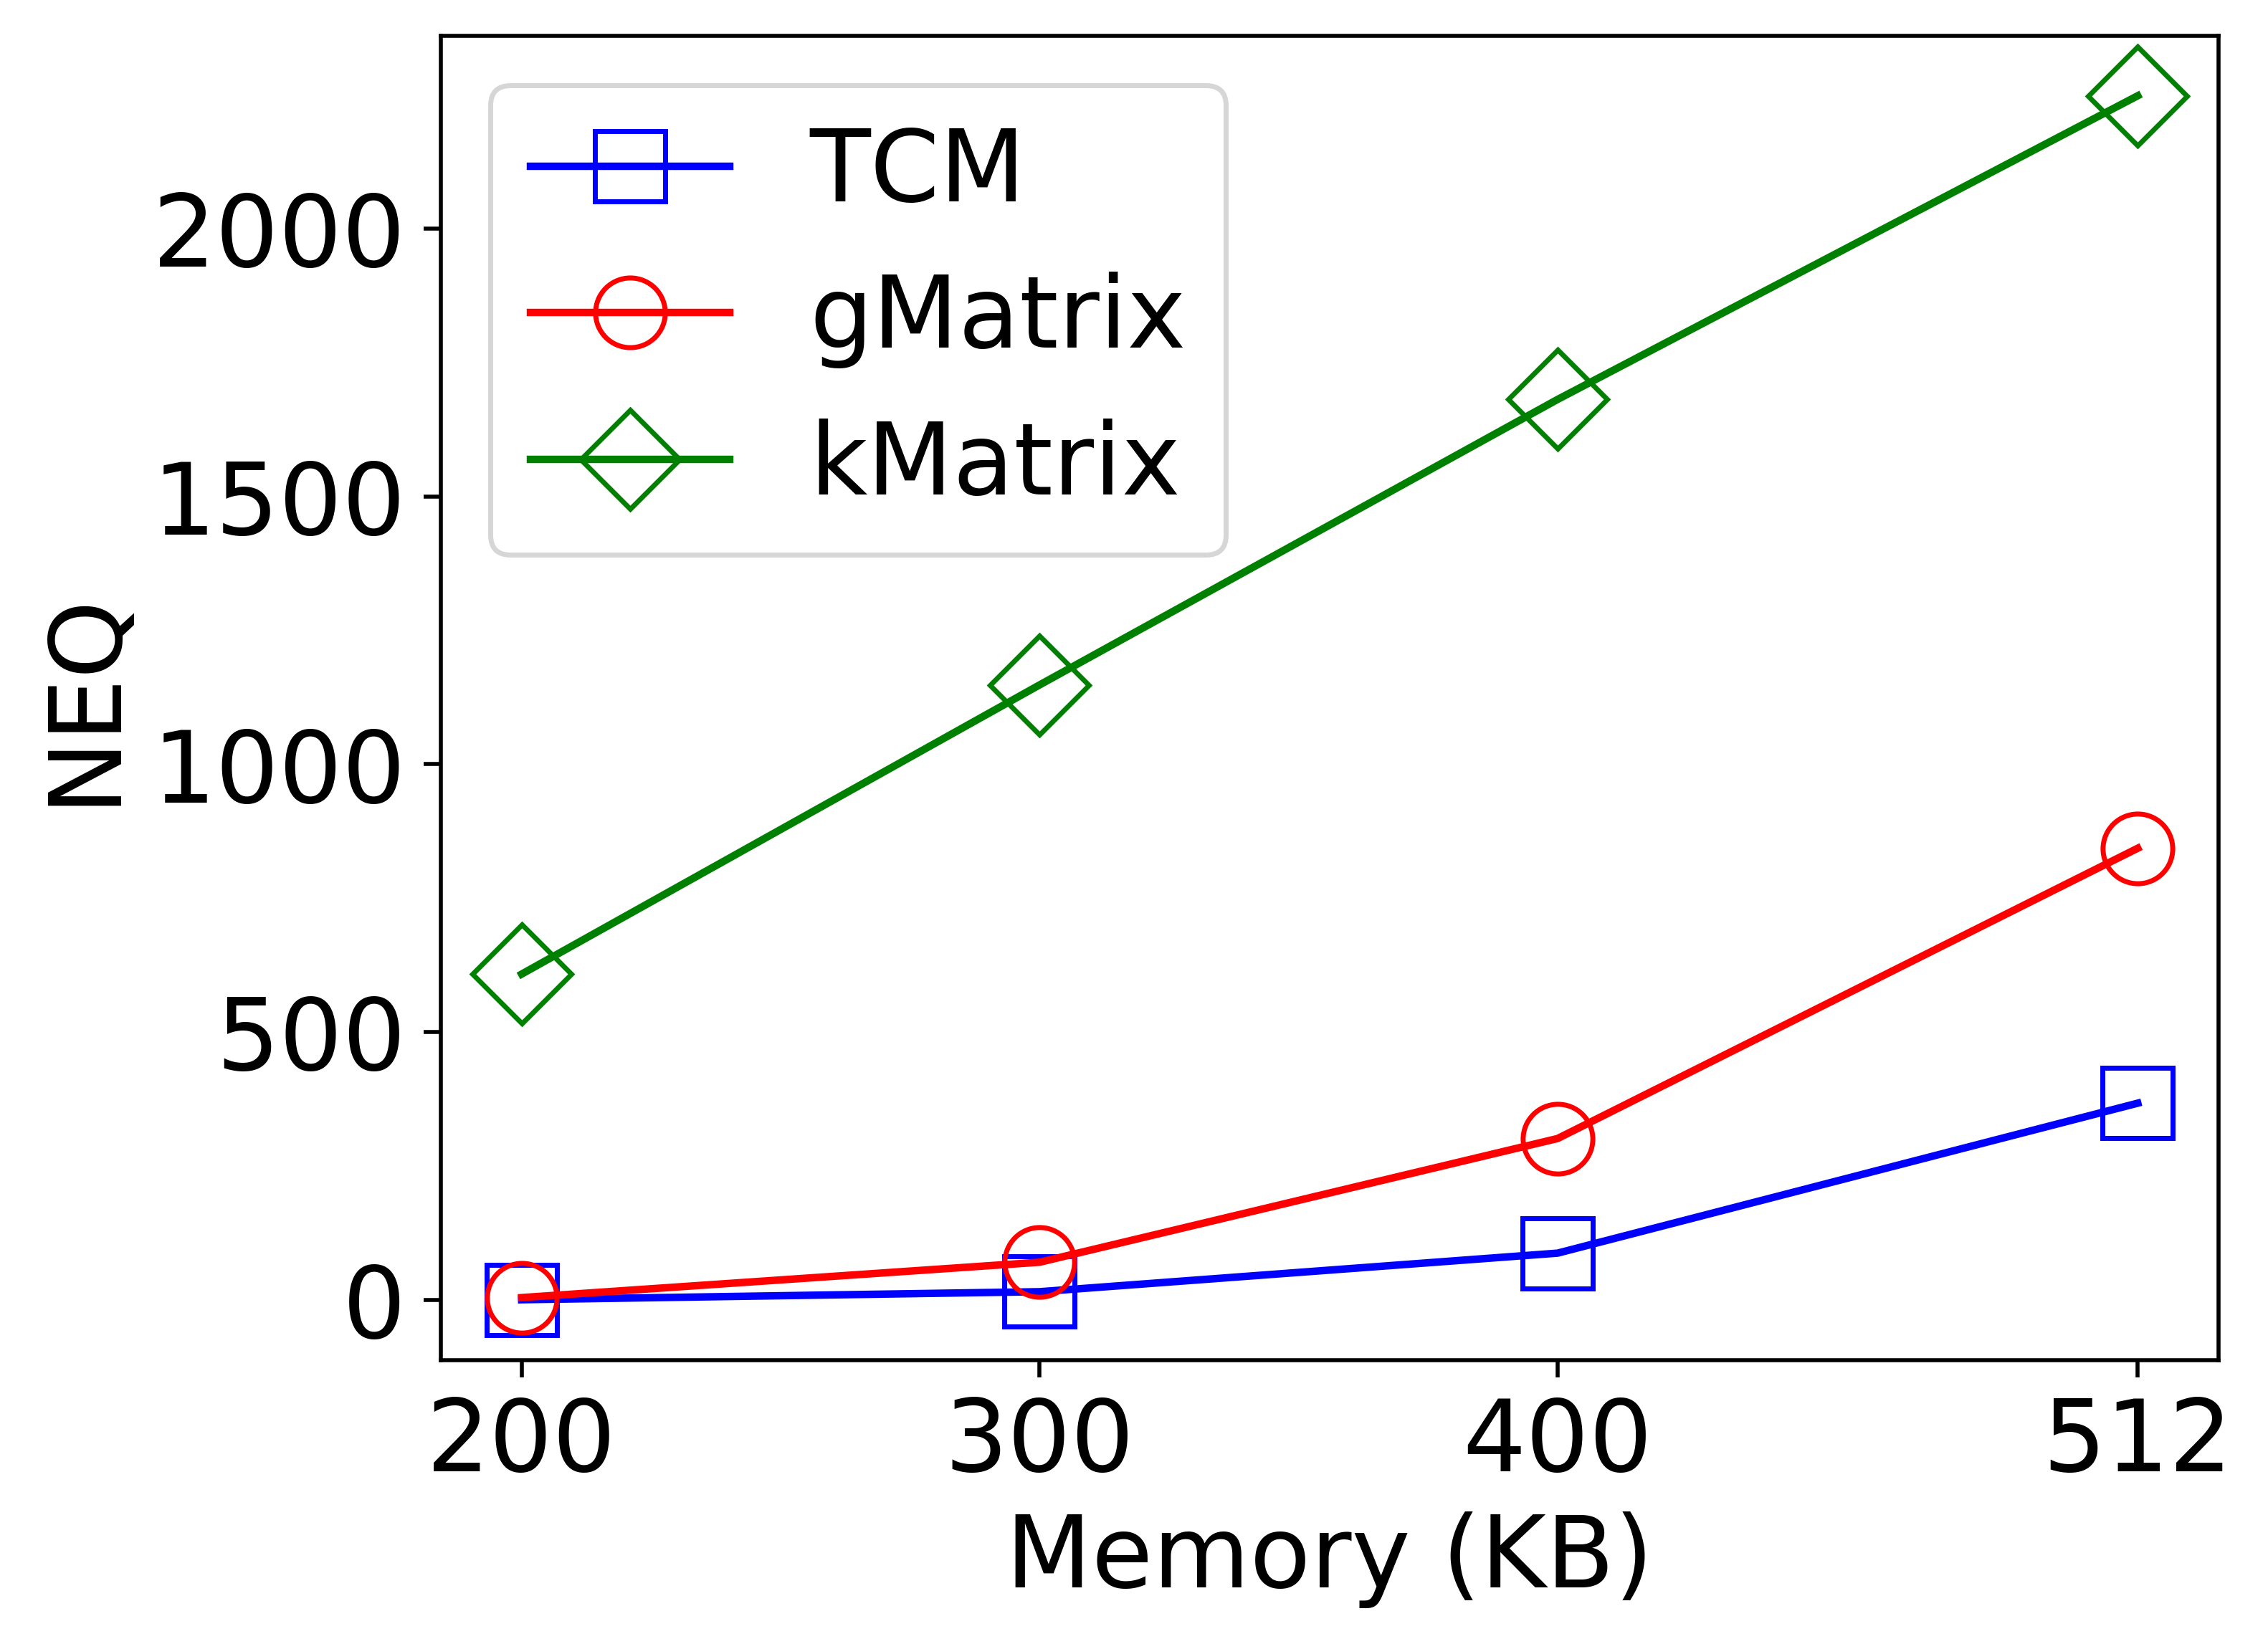
\includegraphics[width=0.45\linewidth]{img/edge_query_neq_unicorn-wget.png}}
    \hfill
    \subfloat[email-EuAll\label{fig:neq-b}]{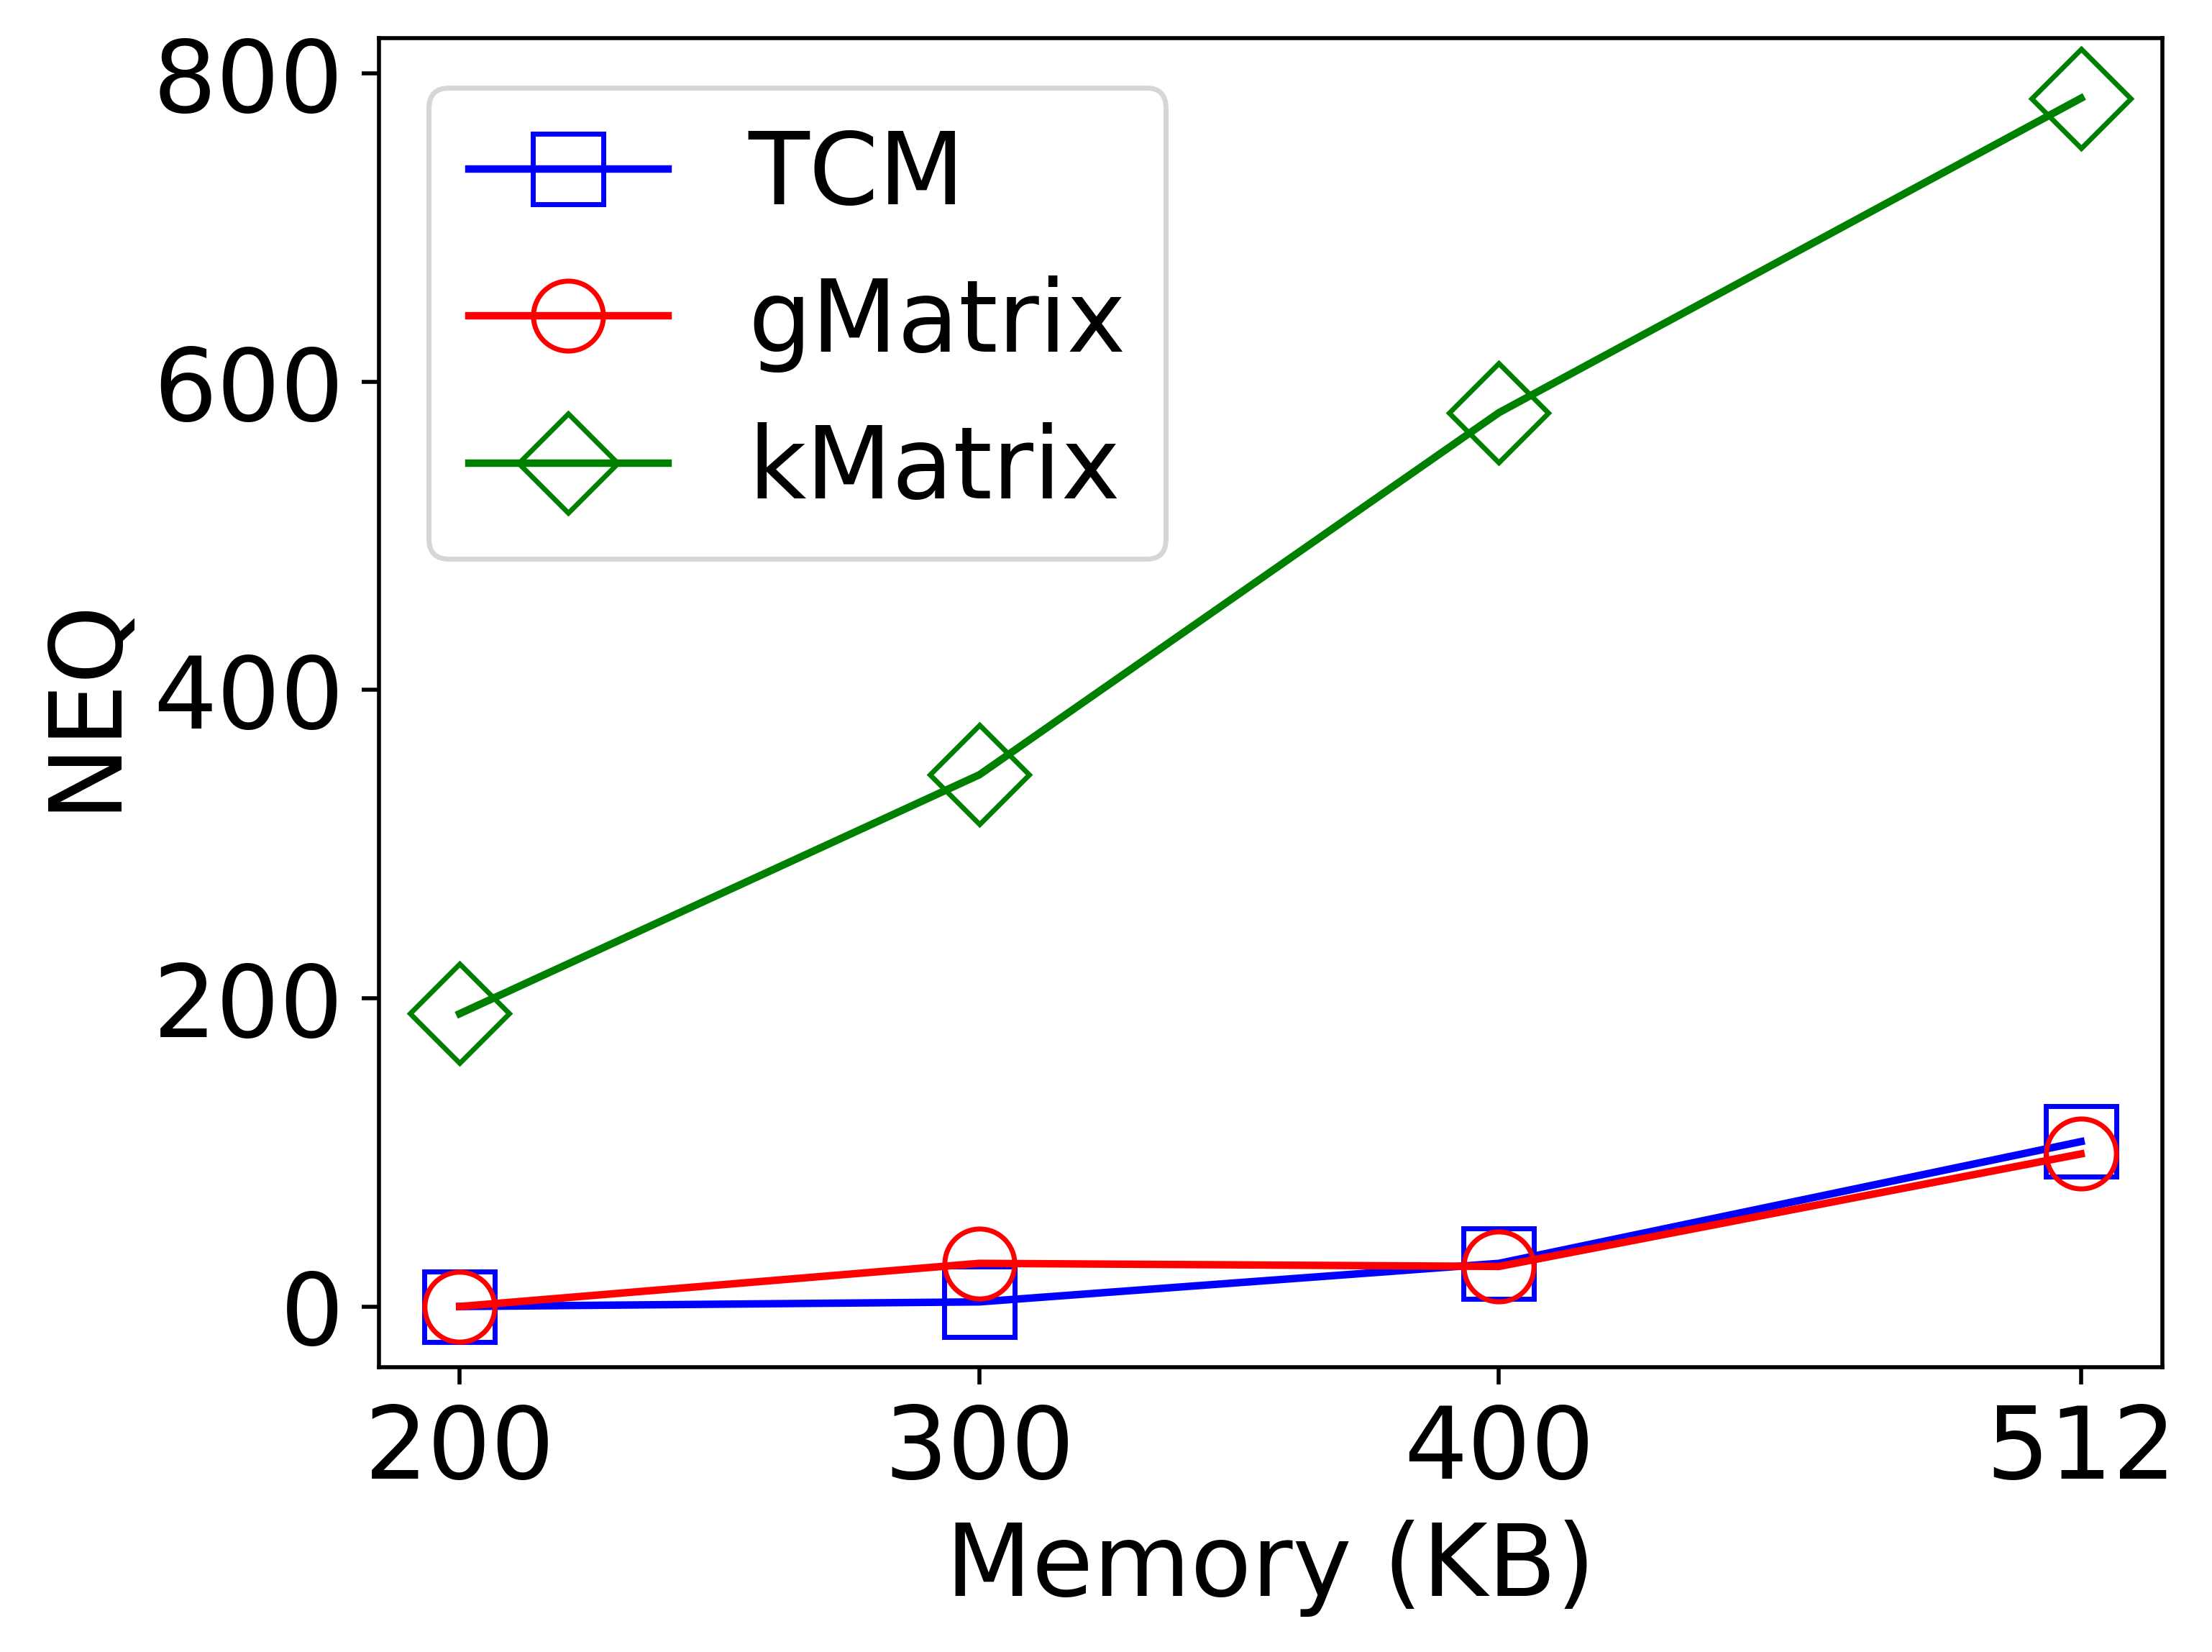
\includegraphics[width=0.45\linewidth]{img/edge_query_neq_email-EuAll.png}}
    \hfill
    \subfloat[cit-HepPh\label{fig:neq-c}]{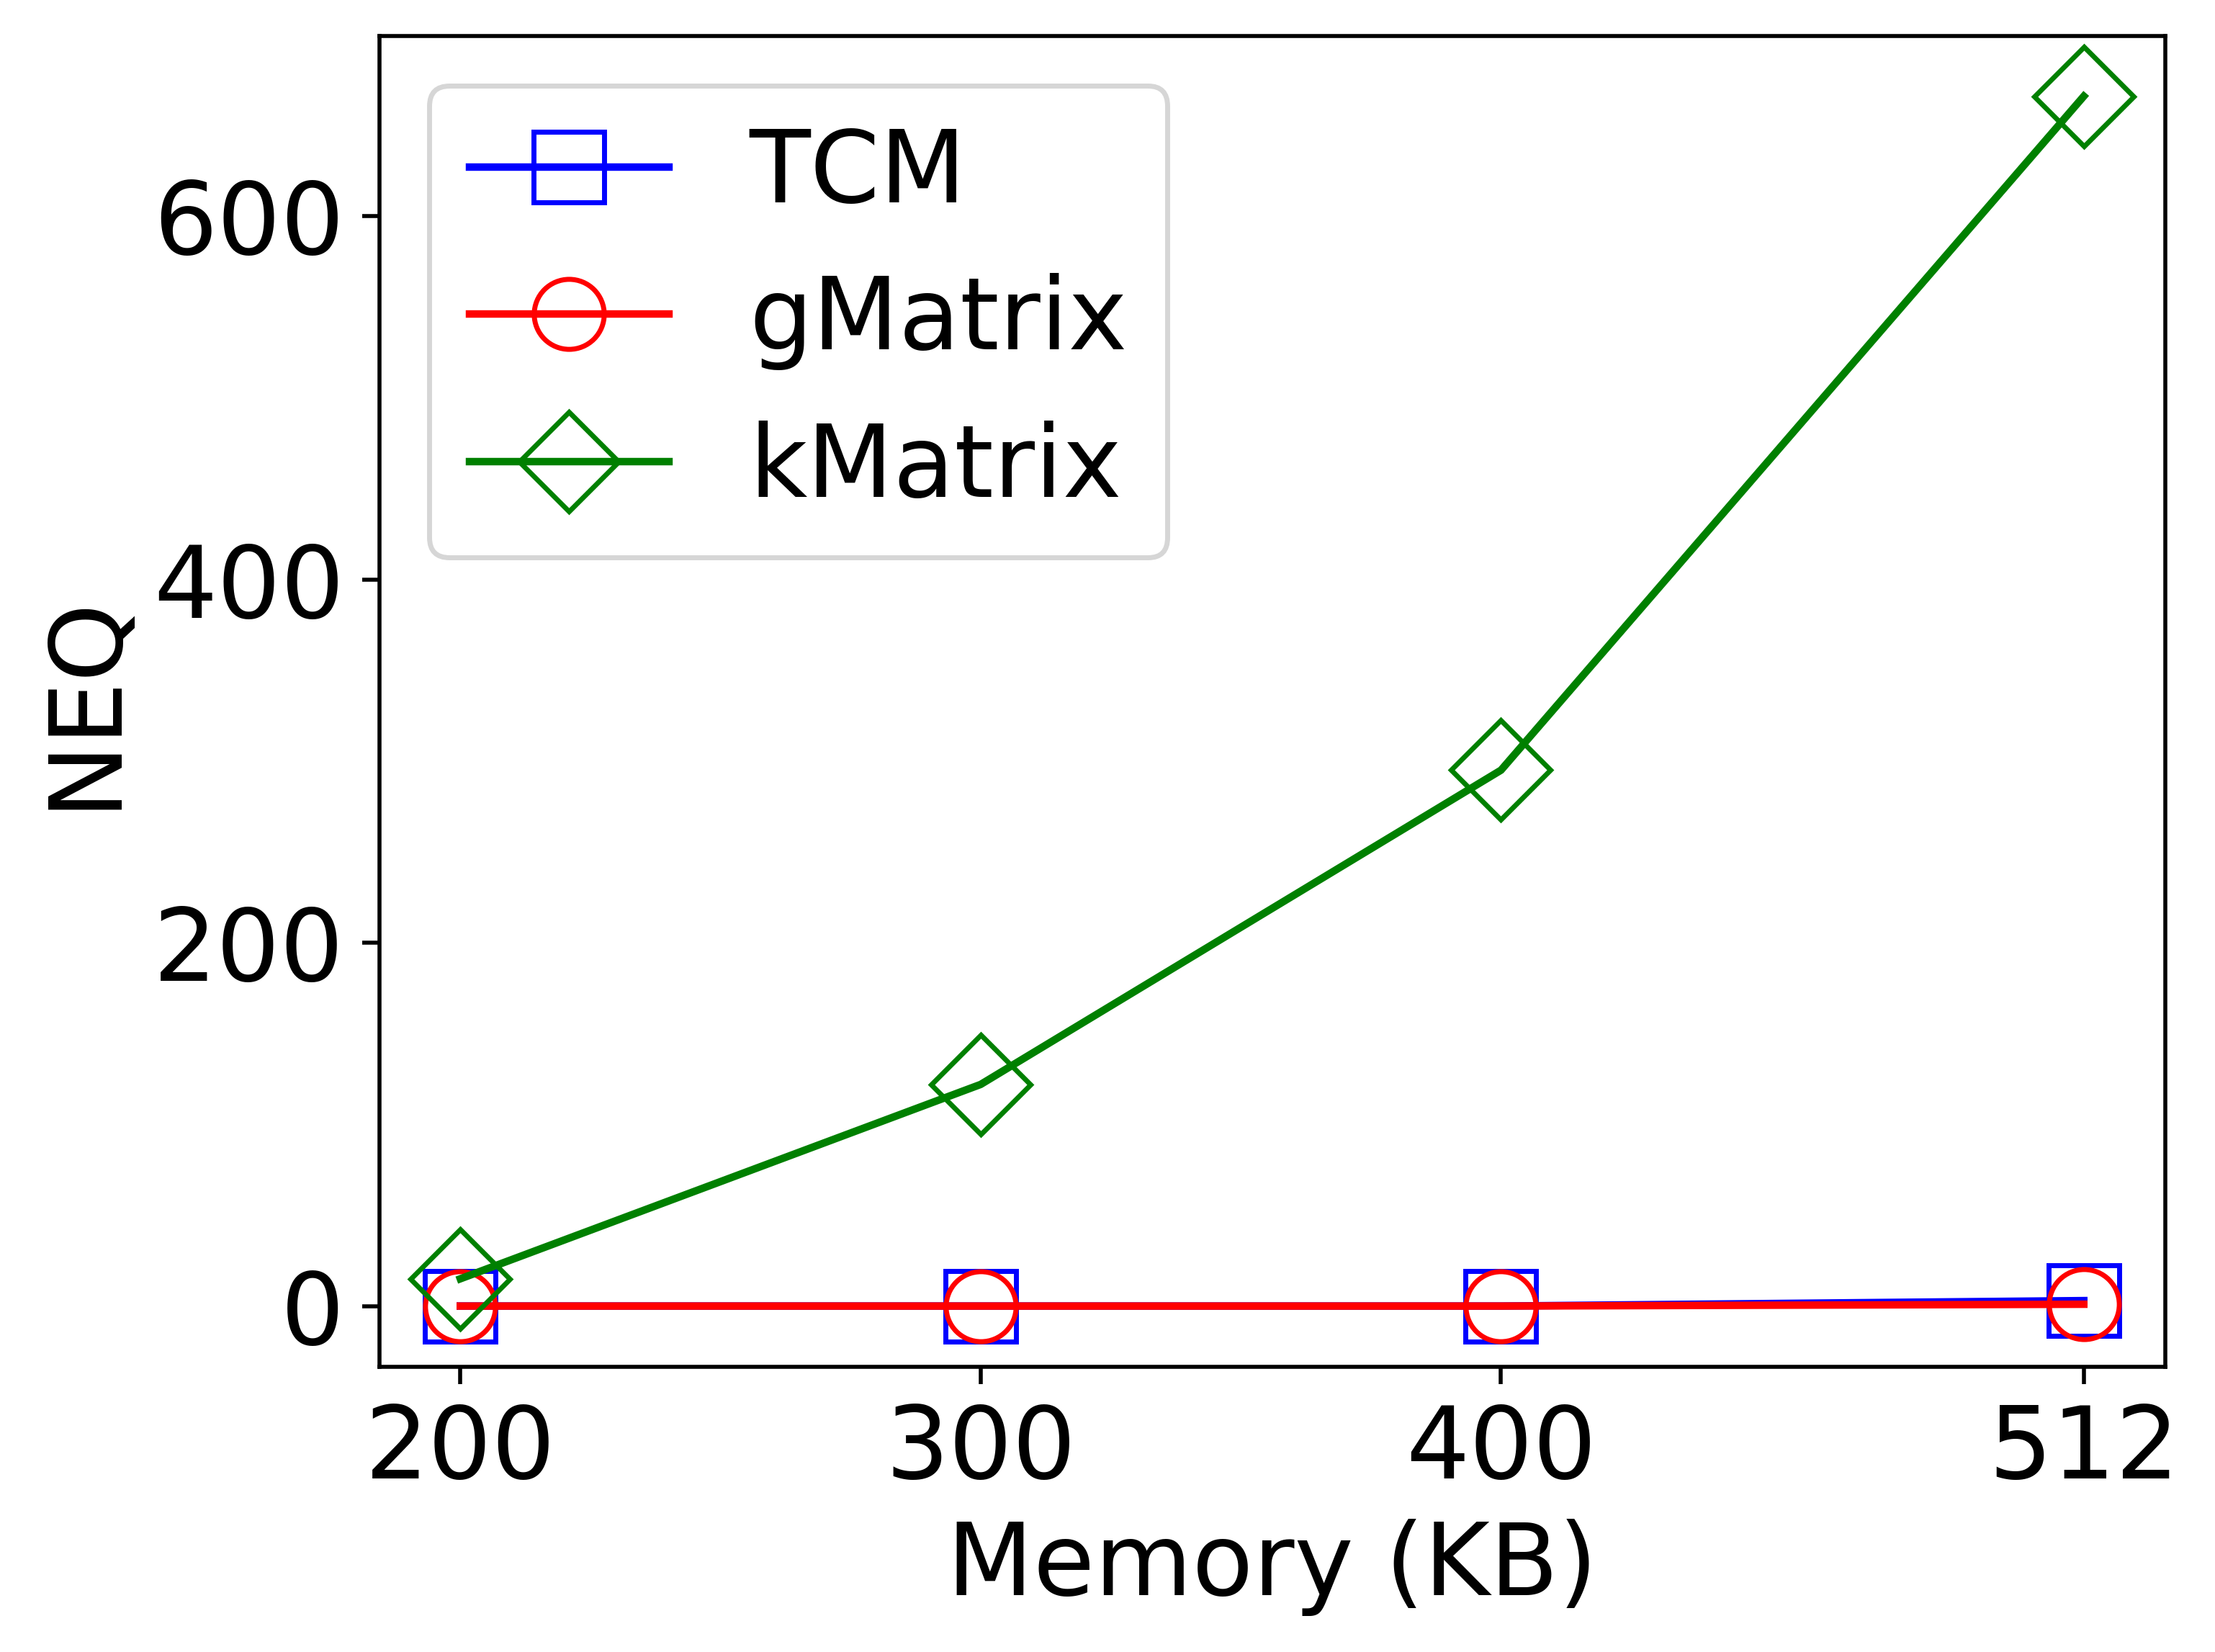
\includegraphics[width=0.45\linewidth]{img/edge_query_neq_cit-HepPh.png}}
    \caption{Number of effective queries}
    \label{fig:edgq-queries-neq-test}
\end{figure}

The number of effective queries for each sketch was calculated by querying the sketches against 10,000 edges chosen through reservoir sampling from the original dataset. kMatrix has surpassed the accuracy of both TCM and gMatrix for all the scenarios that we have tested. The results for cit-HepPh in Fig.~\ref{fig:neq-c} shows that kMatrix has been able to effectively answer a significantly larger number of queries where the other sketches failed due to hash collisions.  